\documentclass[12pt]{article}

% Автор: Илья Дудников
% Автор стиля: Сергей Копелиович

\usepackage{cmap}
\usepackage[T2A]{fontenc}
\usepackage[utf8]{inputenc}
\usepackage[russian]{babel}
\usepackage{graphicx}
\usepackage{amsthm,amsmath,amssymb}
\usepackage{listings}
\usepackage{color}
\usepackage{array}
\usepackage{epigraph}
\usepackage{multicol}
\usepackage{cancel}
\usepackage{float}
\usepackage{wrapfig}
\usepackage{caption}
\usepackage{subcaption}

\usepackage[usenames,dvipsnames]{xcolor}
\usepackage[russian,colorlinks=true,urlcolor=red,linkcolor=blue]{hyperref}
\usepackage{enumerate}
\usepackage{datetime}
\usepackage{fancyhdr}
\usepackage{lastpage}
\usepackage{verbatim}
\usepackage{tikz}
\usepackage{MnSymbol}
\usetikzlibrary{arrows,decorations.markings,decorations.pathmorphing}
\usepackage{pgfplots}
\usepackage{ifthen}
\usepackage{mathtools}
\usepackage{svg}
\usepackage{mathrsfs}

%\usepackage{tabls}
%\usepackage{tabularx}
%\usepackage{xifthen}
%\listfiles

\def\NAME{Ответы на билеты}
\def\SEASON{Алгоритмы и анализ сложности, ПИ, 3 семестр}

\sloppy
\voffset=-20mm
\textheight=235mm
\hoffset=-22mm
\textwidth=180mm
\headsep=12pt
\footskip=20pt

\parskip=0em
\parindent=0em

\setlength\epigraphwidth{.8\textwidth}

\newlength{\tmplen}
\newlength{\tmpwidth}
\newcounter{listcounter}

% Список с маленькими отступами
\newenvironment{MyList}[1][4pt]{
  \begin{enumerate}[1.]
  \setlength{\parskip}{0pt}
  \setlength{\itemsep}{#1}
}{       
  \end{enumerate}
}
% Вложенный список с маленькими отступами
\newenvironment{InnerMyList}[1][0pt]{
  \vspace*{-0.5em}
  \begin{enumerate}[(a)]
  \setlength{\parskip}{-0pt}
  \setlength{\itemsep}{#1}
}{       
  \end{enumerate}
  \vspace*{-0.5em}
}
% Список с маленькими отступами
\newenvironment{MyItemize}[1][4pt]{
  \begin{itemize}
  \setlength{\parskip}{0pt}
  \setlength{\itemsep}{#1}
}{       
  \end{itemize}
}

% Основные математические символы
\def\TODO{{\color{red}\bf TODO}}
\def\C{\mathbb{C}}       %
\def\Q{\mathbb{Q}}       %
\def\N{\mathbb{N}}       %
\def\R{\mathbb{R}}       %
\def\F2{\mathbb{F}_2}    %
\def\Z{\mathbb{Z}}       %
\def\INF{\t{+}\infty}    % +inf
\def\EPS{\varepsilon}    %
\def\EMPTY{\varnothing}  %
\def\PHI{\varphi}        %
\def\SO{\Rightarrow}     % =>
\def\EQ{\Leftrightarrow} % <=>
\def\t{\texttt}          % mono font
\def\c#1{{\rm\sc{#1}}}   % font for classes NP, SAT, etc
\def\O{\mathcal{O}}      %
\def\NO{\t{\#}}          % #
\def\XOR{\text{ {\raisebox{-2pt}{\ensuremath{\Hat{}}}} }}
\renewcommand{\le}{\leqslant}
\renewcommand{\ge}{\geqslant}
\newcommand{\q}[1]{\langle #1 \rangle}               % <x>
\newcommand\URL[1]{{\footnotesize{\url{#1}}}}        %
% \newcommand{\sfrac}[2]{{\scriptscriptstyle\frac{#1}{#2}}}  % Очень маленькая дробь
% \newcommand{\mfrac}[2]{{\scriptstyle\frac{#1}{#2}}}    % Небольшая дробь
\newcommand{\sfrac}[2]{{\scriptstyle\frac{#1}{#2}}}  % Очень маленькая дробь
\newcommand{\mfrac}[2]{{\textstyle\frac{#1}{#2}}}    % Небольшая дробь

\newcommand{\fix}[1]{{\color{fixcolor}{#1}}} % \underline
\def\bonus{\t{\red{(*)}}}
\def\ifbonus#1{\ifthenelse{\equal{#1}{}}{}{\bonus}}
\def\smallsquare{$\scalebox{0.5}{$\square$}$}

\newlength{\myItemLength}
\setlength{\myItemLength}{0.3em}
\def\ItemSymbol{\smallsquare}
\def\Item{\vspace*{\myItemLength}\ItemSymbol \ \ }

\newcommand{\LET}{%
  % [line width=0.6pt]
  \begin{tikzpicture}%
  \draw(0.8ex,0) -- (0.8ex,1.6ex);%
  \draw(0,1.6ex) -- (0.8ex,1.6ex);%
  \end{tikzpicture}%
  \hspace*{0.1em}%
}

% Отступы
\def\makeparindent{\hspace*{\parindent}\unskip}
\def\up{\vspace*{-0.5em}}%{\vspace*{-\baselineskip}}
\def\down{\vspace*{0.5em}}
\def\LINE{\vspace*{-1em}\noindent \underline{\hbox to 1\textwidth{{ } \hfil{ } \hfil{ } }}}
\def\BOX#1{\mbox{\fbox{\bf{#1}}}}
\def\Pagebreak{\pagebreak\vspace*{-1.5em}}

% Мелкий заголовок
\newcommand{\THEE}[1]{
  \vspace*{0.5em}
  \noindent{\bf \underline{#1}}%\hspace{0.5em}
  \vspace*{0.2em}
}
% Другой тип мелкого заголовка
\newcommand{\THE}[1]{
  \vspace*{0.5em} $\bullet$
  \noindent{\bf #1}%\hspace{0.5em}
  \vspace*{0.2em}
}

\newenvironment{MyTabbing}{
  \t\bgroup
  \vspace*{-\baselineskip}
  \begin{tabbing}
    aaaa\=aaaa\=aaaa\=aaaa\=aaaa\=aaaa\kill
}{
  \end{tabbing}
  \t\egroup
}

% Код с правильными отступами
\lstnewenvironment{code}{
  \lstset{}
%  \vspace*{-0.2em}
}%
{
%  \vspace*{-0.2em}
}
\lstnewenvironment{codep}{
  \lstset{language=python}
}%
{
}

% Формулы с правильными отступами
\newenvironment{smallformula}{
 
  \vspace*{-0.8em}
}{
  \vspace*{-1.2em}
  
}
\newenvironment{formula}{
 
  \vspace*{-0.4em}
}{
  \vspace*{-0.6em}
  
}

% Большая квадратная скобка
\makeatletter
\newenvironment{sqcases}{%
  \matrix@check\sqcases\env@sqcases
}{%
  \endarray\right.%
}
\def\env@sqcases{%
  \let\@ifnextchar\new@ifnextchar
  \left\lbrack
  \def\arraystretch{1.2}%
  \array{@{}l@{\quad}l@{}}%
}
\makeatother

% theorems
\makeatother
\usepackage{thmtools}
\usepackage[framemethod=TikZ]{mdframed}
\mdfsetup{skipabove=1em,skipbelow=0em}


\theoremstyle{definition}

\declaretheoremstyle[
    headfont=\bfseries\sffamily\color{ForestGreen!70!black}, bodyfont=\normalfont,
    mdframed={
        linewidth=2pt,
        rightline=false, topline=false, bottomline=false,
        linecolor=ForestGreen, backgroundcolor=ForestGreen!5,
    }
]{thmgreenbox}

\declaretheoremstyle[
    headfont=\bfseries\sffamily\color{NavyBlue!70!black}, bodyfont=\normalfont,
    mdframed={
        linewidth=2pt,
        rightline=false, topline=false, bottomline=false,
        linecolor=NavyBlue, backgroundcolor=NavyBlue!5,
    }
]{thmbluebox}

\declaretheoremstyle[
    headfont=\bfseries\sffamily\color{NavyBlue!70!black}, bodyfont=\normalfont,
    mdframed={
        linewidth=2pt,
        rightline=false, topline=false, bottomline=false,
        linecolor=NavyBlue
    }
]{thmblueline}

\declaretheoremstyle[
    headfont=\bfseries\sffamily\color{RawSienna!70!black}, bodyfont=\normalfont,
    mdframed={
        linewidth=2pt,
        rightline=false, topline=false, bottomline=false,
        linecolor=RawSienna, backgroundcolor=RawSienna!5,
    }
]{thmredbox}

\declaretheoremstyle[
    headfont=\bfseries\sffamily\color{RawSienna!70!black}, bodyfont=\normalfont,
    numbered=no,
    mdframed={
        linewidth=2pt,
        rightline=false, topline=false, bottomline=false,
        linecolor=RawSienna, backgroundcolor=RawSienna!1,
    },
    qed=\qedsymbol
]{thmproofbox}

\declaretheoremstyle[
    headfont=\bfseries\sffamily\color{NavyBlue!70!black}, bodyfont=\normalfont,
    numbered=no,
    mdframed={
        linewidth=2pt,
        rightline=false, topline=false, bottomline=false,
        linecolor=NavyBlue, backgroundcolor=NavyBlue!1,
    },
]{thmexplanationbox}

\declaretheorem[style=thmgreenbox, name=Определение]{Def}
\declaretheorem[style=thmbluebox, numbered=no, name=Пример]{Example}
\declaretheorem[style=thmredbox, name=Утверждение]{Prop}
\declaretheorem[style=thmredbox, name=Теорема]{Thm}
\declaretheorem[style=thmredbox, name=Свойство]{Property}
\declaretheorem[style=thmredbox, name=Лемма]{Lm}
\declaretheorem[style=thmredbox, numbered=no, name=Следствие]{Cons}

\declaretheorem[style=thmproofbox, name=Доказательство]{replacementproof}
\renewenvironment{proof}[1][\proofname]{\vspace{-10pt}\begin{replacementproof}}{\end{replacementproof}}


\declaretheorem[style=thmexplanationbox, name=Доказательство]{tmpexplanation}
\newenvironment{explanation}[1][]{\vspace{-10pt}\begin{tmpexplanation}}{\end{tmpexplanation}}

\declaretheorem[style=thmblueline, numbered=no, name=Замечание]{Rem}
\declaretheorem[style=thmblueline, numbered=no, name=Note]{note}
\declaretheorem[style=thmblueline, numbered=no, name=Обозначение]{notation}

% \newtheorem*{notation}{Notation}
\newtheorem*{Ex}{Упражнение}

% Определяем основные секции: \begin{Lm}, \begin{Thm}, \begin{Def}, \begin{Rem}
% \renewcommand{\qedsymbol}{$\blacksquare$}
% \theoremstyle{definition} % жирный заголовок, плоский текст
% \newtheorem{Thm}{\underline{Теорема}}[subsection] % нумерация будет "<номер subsection>.<номер теоремы>"
% \newtheorem{Lm}[Thm]{\underline{Lm}} % Нумерация такая же, как и у теорем
% \newtheorem{Ex}[Thm]{Упражнение} % Нумерация такая же, как и у теорем
% \newtheorem{Example}[Thm]{Пример} % Нумерация такая же, как и у теорем
% \newtheorem{Code}[Thm]{Код} % Нумерация такая же, как и у теорем
% \theoremstyle{plain} % жирный заголовок, курсивный текст
% \newtheorem{Def}[Thm]{Def} % Нумерация такая же, как и у теорем
% \theoremstyle{remark} % курсивный заголовок, плоский текст
% \newtheorem{Cons}[Thm]{Следствие} % Нумерация такая же, как и у теорем
% \newtheorem{Conj}[Thm]{Гипотеза} % Нумерация такая же, как и у теорем
% \newtheorem{Prop}[Thm]{Утверждение} % Нумерация такая же, как и у теорем
% \newtheorem{Rem}[Thm]{Замечание} % Нумерация такая же, как и у теорем
% \newtheorem{Remark}[Thm]{Замечание} % Нумерация такая же, как и у теорем
% \newtheorem{Algo}[Thm]{Алгоритм} % Нумерация такая же, как и у теорем

% Определяем ЗАГОЛОВКИ
\def\SectionName{unknown}
\def\AuthorName{unknown}

\newlength{\sectionvskip}
\setlength{\sectionvskip}{0.5em}
\newcommand{\Section}[4][]{
  % Заголовок
  \pagebreak
%  \ifthenelse{\isempty{#1}}{
    \refstepcounter{section}
%  }{}
  \vspace{0.5em}
%  \ifthenelse{\isempty{#1}}{
%    \addtocontents{toc}{\protect\addvspace{-5pt}}%
    \addcontentsline{toc}{section}{\arabic{section}. #2}
%  }{}
  \begin{center}
    {\Large \bf Раздел \NO{\arabic{section}}: #2} \\ 
    \vspace{\sectionvskip}
    \ifthenelse{\equal{#3}{}}{}{{\large #3}\\}
  \end{center}

  \LINE

  % Запомнили название и автора главы
  \gdef\SectionName{#2}
  \gdef\AuthorName{#4}

  % Заголовок страницы
  \lhead{\SEASON}
  \chead{}
  \rhead{\SectionName}
  \renewcommand{\headrulewidth}{0.4pt}

  \lfoot{Глава \NO{\arabic{section}}.}
  \cfoot{\thepage\t{/}\pageref*{LastPage}}
  \rfoot{Автор: \AuthorName}
  \renewcommand{\footrulewidth}{0.4pt}
}

\newcommand{\Subsection}[2][]{
  \refstepcounter{subsection}
  \vspace*{1em}
  \ifthenelse{\equal{#1}{}}
    {\addcontentsline{toc}{subsection}{\arabic{section}.\arabic{subsection}. #2}}
    {\addcontentsline{toc}{subsection}{\arabic{section}.\arabic{subsection}. \bonus\,#2}}
  {\color{blue}\bf\large \arabic{section}.\arabic{subsection}. \ifbonus{#1}\,{#2}} 
  \vspace*{0.5em}
  \makeparindent
}
\newcommand{\Subsubsection}[2][]{
  \refstepcounter{subsubsection}
  \vspace*{1em}
  \ifthenelse{\equal{#1}{}}
    {\addcontentsline{toc}{subsubsection}{\arabic{section}.\arabic{subsection}.\arabic{subsubsection}. #2}}
    {\addcontentsline{toc}{subsubsection}{\arabic{section}.\arabic{subsection}.\arabic{subsubsection}. \bonus\,#2}}
  {\color{blue}\bf\large \arabic{section}.\arabic{subsection}.\arabic{subsubsection}. \ifbonus{#1}\,#2}
  \vspace*{0.5em}
  \makeparindent
}

\makeatletter
\newcommand*{\encircled}[1]{\relax\ifmmode\mathpalette\@encircled@math{#1}\else\@encircled{#1}\fi}
\newcommand*{\@encircled@math}[2]{\@encircled{$\m@th#1#2$}}
\newcommand*{\@encircled}[1]{%
  \tikz[baseline,anchor=base]{\node[draw,circle,outer sep=0pt,inner sep=.2ex] {#1};}}
\makeatother

\newcommand{\Header}{
  \pagestyle{empty}
  \renewcommand{\dateseparator}{--}
  \begin{center}
    {\Large\bf 
     Алгоритмы и анализ сложности, 3 семестр ПИ,\\
    \vspace{0.3em}
    \NAME}\\
    \vspace{0.7em}
    {Собрано {\today} в {\currenttime}}
  \end{center}

  \LINE
  \vspace{0em}

  \renewcommand{\baselinestretch}{0.98}\normalsize
  \tableofcontents
  \renewcommand{\baselinestretch}{1.0}\normalsize
  \pagebreak
}

\newcommand{\BeginConspect}{
  \pagestyle{fancy}
  \setcounter{page}{1}
}

\definecolor{mygray}{rgb}{0.7,0.7,0.7}
\definecolor{ltgray}{rgb}{0.9,0.9,0.9}
\definecolor{fixcolor}{rgb}{0.7,0,0}
\definecolor{red2}{rgb}{0.7,0,0}
\definecolor{dkred}{rgb}{0.4,0,0}
\definecolor{dkblue}{rgb}{0,0,0.6}
\definecolor{dkgreen}{rgb}{0,0.6,0}
\definecolor{brown}{rgb}{0.5,0.5,0}

\newcommand{\green}[1]{{\color{green}{#1}}}
\newcommand{\black}[1]{{\color{black}{#1}}}
\newcommand{\red}[1]{{\color{red}{#1}}}
\newcommand{\dkred}[1]{{\color{dkred}{#1}}}
\newcommand{\blue}[1]{{\color{blue}{#1}}}
\newcommand{\dkgreen}[1]{{\color{dkgreen}{#1}}}

\newcommand{\Mod}[1]{\ (\mathrm{mod}\ #1)}

\DeclareMathOperator{\Real}{Re}
\DeclareMathOperator{\Imag}{Im}
\DeclareMathOperator{\lcm}{lcm}
\DeclareMathOperator{\sign}{sign}
\DeclareMathOperator{\Si}{Si}
\DeclareMathOperator{\const}{const}
\DeclareMathOperator{\Arg}{Arg}
\DeclareMathOperator{\Int}{Int}
\DeclareMathOperator{\Cl}{Cl}
\DeclareMathOperator{\diam}{diam}

\begin{document}
    \Header

    \BeginConspect

    \Section{Вопрос 1}{}{Гагин Артур}
    
    \Subsection{Машины Тьюринга и тезис Чёрча}
   
    \begin{Def}[Машина Тьюринга]
        Да что за <<Машина Тьюринга>>?
        \begin{itemize}
            \item Абстрактная вычислительная машина.
            \item Формализация понятия алгоритма.
            \item Расширение конечного автомата.
            \item Лента (бесконечная).
            \item Головка записи-чтения (управляющее устройство), способная находиться в одном из множества состояний, которое конечно и точно задано.
            \item Это управляющее может перемещаться влево и вправо по ленте, читать и записывать в ячейки символы некоторого конечного алфавита.
            \item Существует $\epsilon$-символ, который заполняет все пустые клетки ленты.
            \item Управляющее устройство работает согласно правилам перехода, которые представляют алгоритм, реализуемый данной МТ. Каждое правило перехода предписывает машине, в зависимости от текущего состояния и наблюдаемого в текущей ячейке символа, записать в эту клетку новый символ, перейти в новое состояние и переместиться на одну клетку влево или вправо (существует некий <<синтаксический сахар>> --- остаться на месте). Некоторые состояния могут быть помечены как терминальные, и переход в любое из них означает конец работы, остановку алгоритма.
        \end{itemize}
        Это все очень интересно, но как насчет формализма?\\
        Формально: $M = \{Q, G, \epsilon, \Sigma, \delta, q_0, F\}$ --- запомните этот набор из семи элементов!
        \begin{itemize}
        \item $Q$ --- конечное, не являющееся пустым, множество состояний.
        \item $G$ --- конечный, не являющийся пустым, набор символов ленточного алфавита.
        \item $\epsilon$ --- единственный пустой символ.
        \item $\Sigma = G \backslash \{\epsilon\}$ --- набор входных символов.
        \item $\delta : (Q \backslash F) \times G \bcancel{\rightarrow}
        Q \times G \times \{L, R\}$ --- частичная функция, называемая функцией перехода, где $L$ --- сдвиг влево, а $R$ --- сдвиг вправо. Если $\delta$ не определена для текущего состояния и символа ленты, то машина останавливается.
        \item $q_0$ --- это начальное состояние.
        \item $F \subset {Q}$  --- набор конечных состояний.
        \end{itemize}
    \end{Def} 
    \begin{Rem}
        А что если мы хотим такое состояние, которое будет являться term при одном символе на ленте и nonterm при другом символе?\\
        Если немного подумать, то здесь все в порядке, поскольку мы можем сделать это состояние nonterm, перейти в другое term состояние, а при определенном символе сдвинуться, например, вправо, записав на ленту такой же символ, что был на ней.
    \end{Rem}
    \begin{Rem}
        Хоть любой конечный алфавит и не ограничен одними цифрами 0 и 1, очевидно, что мы всегда можем его представить в виде двоичных чисел, введя на нем порядок.
    \end{Rem}
    \begin{Def}[Частичная функция]
        частичная функция $f$ из множества $X$ в множество Y --- это функция из подмножества $S$ из $X$ (возможно, самого $X$) в $Y$ (обозначение: $\bcancel{\rightarrow}$). 
    \end{Def}
    \begin{Def}[Детерминированная и недетерминированная машины Тьюринга]
        Машина Тьюринга называется детерминированнй, если каждой паре состояни и ленточного символа соответствует не более одного правила. В ином случае, машина является недетерминированной.
    \end{Def}
    \begin{Def}[Тезис Черча/Тьюринга/Черча-Тьюринга]
        Есть ли отличие?\\
        На самом деле, все они говорят об одном, просто Черч в свое время придумал $\lambda$-исчисления, Тьюринг придумал Машину Тьюринга, а позже было показано, что эти формализмы эквивалентны.\\
        Сам тезис сформулируем следующим образом: Класс алгоритмически вычислимых частичных функций совпадает с классом всех функций, вычислимых на машине Тьюринга.
    \end{Def}
    \begin{Rem}
        Стоит понимать, что это именно тезис, а не теорема, ведь понятие <<алгоритмически вычислимая частичная функция>> неформально.
    \end{Rem}
    \begin{Def}[Вычислимая функция] 
        Вычислимые функции — это множество функций вида, $ f \colon N\ \to N $, которые могут быть реализованы на машине Тьюринга.\\
        В качестве множества $N$ обычно рассматривается множество $B^{*}$ — множество слов в двоичном алфавите $B = \{0,1\}$, с оговоркой, что результатом вычисления может быть не только слово, но и специальное значение «неопределённость», соответствующее случаю, когда алгоритм «зависает». Таким образом, можно дать следующее определение $N$:\\
        $N=B^{*}\cup \{\operatorname{undef} \}$, где $B=\{0,1\}$, а $\operatorname{undef}$ — специальный элемент, означающий неопределённость.\\
        Роль множества $N$ может играть множество натуральных чисел, к которому добавлен элемент $ \operatorname{undef} $, и тогда вычислимые функции --- это некоторое подмножество натуральнозначных функций натурального аргумента. Удобно считать, что в качестве $N$ могут выступать различные счётные множества --- множество натуральных чисел, множество рациональных чисел, множество слов в каком-либо конечном алфавите и др. 
    \end{Def}
    
    \Subsection{Классы RE, R и co-RE, доказательство R $=$ RE $\cap$ co-RE}
    
    \begin{Def}[Классы RE и co-RE]
        Класс RE (recursively enumerable) --- класс decision problems (проблемы принятия решения), для которых ответ <<да>> может быть проверен машиной Тьюринга за конечное время.
        \begin{itemize}
            \item Если на проблему ответ <<да>>, то существует некоторая процедура, которая требует конечного времени для определения этого.
            \item Ложь здесь отсутствует.
            \item Если на проблему ответ <<нет>>, то машина Тьюринга может остановиться, а может и не остановиться.
        \end{itemize}
        Класс co-RE является дополнением к классу RE: ответ <<нет>> можно получить за конечное время абсолютно всегда, получение противоположного ответа может занять вечность.
    \end{Def}
    \begin{Def}[Формальный язык]
        Формальный язык (или просто язык) --- это множество конечных слов над конечным алфавитом.
    \end{Def}
    \begin{Def}[Класс R]
        R --- класс decision problems, решаемых на МТ (набор всех рекурсивных языков). 
    \end{Def}
    \begin{Def}[Рекурсивный язык] 
        Формальный язык является рекурсивным, если существует полная машина Тьюринга (машина Тьюринга, которая останавливается для каждого заданного ввода), которая, когда на вход подается конечная последовательность символов, принимает ее, если она принадлежит языку, и отвергает ее в противном случае. 
    \end{Def}
    \begin{Thm}
        R $=$ RE $\cap$ co-RE.
    \end{Thm}
    \begin{proof}
        Обозначим за $X$ класс decision problems, содержащихся в классе RE, ответы <<да>> и <<нет>> на которые можно получить за конечное время. Очевидно, что $X$ $\subset$ co-RE по определению, а также никакая другая задача, содержащаяся в RE не содержится в co-RE. То есть, $X$ $=$ RE $\cap$ co-RE. Однако $X$ $=$ R, так как это в точности класс decision problems, решаемых на машине Тьюринга, то есть: R $=$ $X$ $=$ RE $\cap$ co-RE.
    \end{proof}
    
    \Subsection{Проблемы Acceptance, Halting, Emptiness}
    
    \begin{Def}[Halting Problem]
        Имеется произвольная машина Тьюринга и произвольные входные данные для нее. Вопрос заключается в следующем: возможно ли разработать алгоритм, который точно скажет, останавливается ли эта машина Тьюринга или нет?
    \end{Def}
    \begin{Thm}
        Проблема останова является алгоритмически неразрешимой задачей.
    \end{Thm}
    \begin{proof}
         Доказательство этой проблемы достаточно просто объяснил А.В. Спивак в следующем видео:
        \href{https://www.youtube.com/watch?v=JDWM6tL5oPs&ab_channel=Vanechki%3A%D0%BC%D0%B0%D1%82%D0%B5%D0%BC%D0%B0%D1%82%D0%B8%D0%BA%D0%B0%2C%D0%B1%D0%B8%D0%BE%D0%BB%D0%BE%D0%B3%D0%B8%D1%8F%D0%B8%D0%BC%D0%BD%D0%BE%D0%B3%D0%BE%D0%B5%D0%B4%D1%80%D1%83%D0%B3%D0%BE%D0%B5}{ссылка}.
    \end{proof}
    \begin{Def}[Acceptance problem]
        Имеется произвольная машина Тьюринга и произвольные входные данные для нее. Вопрос заключается в следующем: возможно ли разработать алгоритм, который точно скажет, принимает ли эта машина Тьюринга входные данные, либо же отвергает их.
    \end{Def}
    \begin{Thm}
        Проблема принятия является алгоритмически неразрешимой задачей.
    \end{Thm}
    \begin{proof}
        Пусть у нас есть $ACCEPT_{TM}$:
        $$ACCEPT_{TM} = \{(<M>, s ) | \text{ Машина Тьюринга } M \text{ принимает } s\}.$$
        Поскольку, по предположению, $ACCEPT_{TM}$ вычислима, должна существовать некоторая машина Тьюринга $A$, которая ее решает. 
        Теперь построим программу (машину Тьюринга) $X$, которая принимает в качестве своего единственного аргумента какую-либо МТ следующим образом:\\
        $X(<M>)$ уходит в бесконечный цикл, только если
        $A$ возвращает true на вход $(<M>, <M>)$ (иначе возвращаем true).\\
        Если $X$ принимает $<X>$, то $A$ говорит, что она не принимает $<X>$. Если $X$ не принимает $<X>$, то $A$ опять говорит обратное. Противоречие.
    \end{proof}
    \begin{Def}[Emptiness problem]
        Имеется произвольная машина Тьюринга $M$, где $L(M) \neq \emptyset$ (язык не пуст). Вопрос заключается в следующем: верно ли, что эта машина принимает хотя бы одну строку?
    \end{Def}
    \begin{Thm}
        Проблемы пустоты является алгоритмически неразрешимой задачей.
    \end{Thm}
    \begin{proof}
        Оставляем доказательство данной проблемы в качестве упражнения читателям.
    \end{proof}
    \Section{Вопрос 2}{}{Панкратов Илья}
    
    \Subsection{Совпадение классов языков, распознаваемых ДМТ, МДМТ, НМТ}
    
    \begin{Def}[Детерминированная многоленточная машина Тьюринга]
    $M = \{Q, G, \epsilon, \Sigma, \delta, q_0, F\}$, где
    \begin{itemize}
        \item $Q$ --- конечное, не являющееся пустым, множество состояний.
        \item $G$ --- конечный, не являющийся пустым, набор символов ленточного алфавита.
        \item $\epsilon$ --- единственный пустой символ.
        \item $\Sigma = G \backslash \{\epsilon\}$ --- набор входных символов.
        \item $\delta : (Q \backslash F) \times G^k \bcancel{\rightarrow}
        Q \times (G \times \{L, R\})^k$, где $k$ --- количество лент, $L$ --- сдвиг влево, а $R$ --- сдвиг вправо. Если $\delta$ не определена для текущего состояния и символа ленты, то машина останавливается.
        \item $q_0$ --- это начальное состояние.
        \item $F \subset {Q}$  --- набор конечных состояний.
    \end{itemize}
    \end{Def}
    \begin{Rem}
        Отличие ТМ с одной лентой и $k$-ТМ (ТМ с $k$ лентами) заключается в том, что в функция перехода зависит от $k$ значений на ленте, и переход осуществляет на $k$ лентах сразу.
    \end{Rem}

    % \begin{center}
    %     \begin{figure}
    %         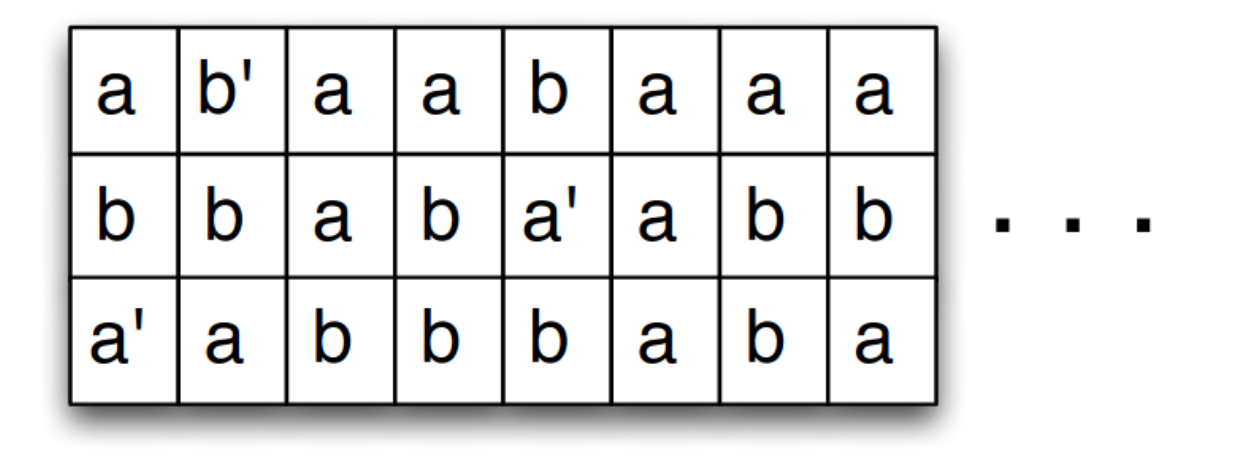
\includegraphics[scale=0.3]{images/k-tape-TM.png}
    %         \caption{ТМ с 3 лентами}
    %         \label{ris:k-tape-TM}
    %     \end{figure}
    % \end{center}

    \begin{Thm}
    Классы языков, распознаваемые детерминированными и многоленточными детерминированными машинами Тьюринга, совпадают.
    \end{Thm}
    \begin{proof}
        \par Однолеточная ТМ --- частный случай ТМ с множеством лент, поэтому нам достаточно свести ТМ с множеством лент к ТМ с одной лентой.
        \par Шаги для сведения $k$-ТМ к $1$-ТМ:
        \begin{itemize}
            \item Записать входные ленты $k$-TM на ленту $1$-TM, разделив ленты \#.
            \item Пометить символы, на которые указывает каждая голова $k$-TM точной (или иным другим символом).
            \item Для исполнения необходимо:
                \begin{itemize}
                    \item Пройти всю ленту $1$-TM, чтобы узнать головы.
                    \item Пройтись с начала ленты $1$-TM, чтобы сделать необходимый переход.
                    \item Если символы головки уходят вправо \#, запишите пробел и сдвиг содержимого ленты.
                \end{itemize}
        \end{itemize}
    \end{proof}

    % \begin{figure}
    %     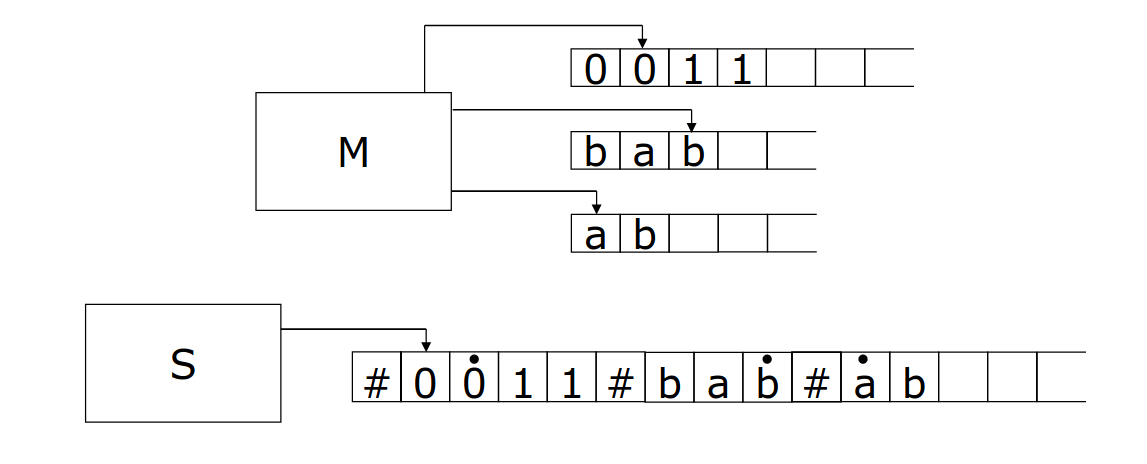
\includegraphics[width=1\linewidth]{images/transform-k-TM-to-1-TM.png}
    %     \caption{Переход от k-TM к 1-TM}
    %     \label{ris:transform}
    % \end{figure}
        
    \begin{Rem}
        Автор полагает, что в данном способе есть недостаток, если ленты на $k$-TM бесконечны. В таком случае можно на ленту $1$-TM записывать данные с лент $k$-TM с помощью кортежей длинны $k$, где каждый $i$ кортеж будет описывать символы на $i$ позиции на каждой ленте.
    \end{Rem}
    \begin{Thm}
    Классы языков, распознаваемые детерминированными и недетерминированными машинами Тьюринга, совпадают.
    \end{Thm}
    \begin{proof}
        \par Мы будем обходить дерево NDTM в ширину, т. к. при обходе в глубину мы бы могли попасть в ветку, в которой зависнем навсегда. Нам нужно сохранять, в какой месте дерева мы сейчас находимся. Для этого мы пронумеруем вершины по порядку на каждом уровне поиска в ширину, и будем записывать последовательность вершин, которую мы выбрали, например, $211$ --- выбрали вторую вершину, затем первую, затем снова первую. И в общем для перевода NDTM в  DTM, нам понадобится три ленты и следующие шаги:
        \begin{enumerate}
            \item Найдём $b$ --- максимальное число недетерминированных выборов, которое мы можем сделать на любом узле (например $2$).
            \item Рассмотрим набор строк, содержащий все числа от $1$ до $b$ $(\sigma = \{1, 2\})$.
            \item Будем проходить по набору, содержащему все возможные комбинации строк из $\sigma$ $\sigma^+ = \{1, 12, 13, ..., 123, ..., 21, ..., 213, ..., b1, ...\}$ ($\sigma^+ = \{1, 2, 11, 12, 21, 22, 111, 112, ...\}$).
            \item Создадим NDT, которая будет выполнять этот алгоритм, принимающая b в качестве входных данных и записывающая члены $\sigma^+$ на свою входную ленту.
        \end{enumerate}
        \par Построим DTM, использующую верхний алгоритм и три ленты, где лены будут отвечать за следующее:
        \begin{enumerate}
            \item Входные данные NDTM.
            \item Отвечает за симуляцию исполнения каждого выбора .
            \item Отвечает за DTM, которая будет строить нам $\sigma^+$.
        \end{enumerate}

        \par Как такая машина будет работать? Будем проходится по следующему алгоритму:
        \begin{enumerate}
            \item Копируем содержимое ленты $1$ на ленту $3$, затем берём путь, сгенерированный на ленте $3$.
            \item Очищаем ленты $2$ и $3$, а затем начинаем алгоритм сначала, пока не исследуем все возможные пути в дереве, если
                \begin{enumerate}
                    \item Закончились пути на $3$ ленте.
                    \item Достигли отклоняющего состояния на второй ленте.
                    \item Если на 3 ленте был сгенерирован путь, которого не существует. Например, у $i$ узла один ребёнок, а путь выглядит так $i2$.
                \end{enumerate}
            \item Если мы встретили только отклоняющие состояние, то отклоняем входные данные, если встретили принимающее состояние, то принимаем входные данные.
        \end{enumerate}
    \end{proof}

    \Section{Вопрос 3}{}{Гагин Артур}
        
    \Subsection{Построение универсальной машины Тьюринга}
    
    \begin{Def}[Универсальная машиина Тьюринга] 
    Универсальная машина Тьюринга --- такая машина, которая может заменить собой любую машину Тьюринга. Получив на вход программу и входные данные, она вычисляет ответ, который вычислила бы по входным данным машина Тьюринга, чья программа была дана на вход.
    \end{Def}
    \begin{Thm}
        Универсальная машина Тьюринга существует.
    \end{Thm}
    \begin{proof}
        Существование УМТ доказывается конструктивно, т.е. явно описывается способ ее построения. Каждая машина Тьюринга вычисляет некоторую фиксированную частично вычислимую функцию из входных строк по своему алфавиту. В этом смысле он ведет себя как компьютер с фиксированной программой. Однако мы можем закодировать таблицу действий любой машины Тьюринга в виде строки. Таким образом, мы можем построить машину Тьюринга, которая ожидает на своей ленте строку, описывающую таблицу действий, за которой следует строка, описывающая входную ленту, и вычисляет ленту, которую вычислила бы закодированная машина Тьюринга. Конкретику оставляем в качестве размышлений читателям.
    \end{proof}
    
    \Subsection{Формулировка теоремы о неразрешимости 10-й Проблемы Гильберта}
    
    \begin{Thm}[10-я проблема Гильберта]
        Не существует алгоритма, который узнавал бы по произвольному диофантову уравнению, имеет ли оно решения в целых числах или нет.
    \end{Thm}
    \begin{Rem}
        Больше о диофантовых уравнениях можно узнать, изучив восьмой вопрос.
    \end{Rem}

    \Subsection{Взаимное сведение 10-й проблемы Гильберта и задачи разрешимости для экзистенциальной арифметики натуральных чисел}
    
    \begin{Def}[Экзистенциальная теория натуральных чисел]
        Экзистенциальная теория чисел из $\N$ --- это множество всех верных утверждений вида 
        $$\exists X_{1} ... \exists X_{n} : E(X_{1}, ..., X_{n}),$$ где $E(X_{1}, ..., X_{n})$ --- это формула без кванторов, в которую входят равенства и неравенства натуральных многочленов.\\
        Предложение этой формы истинно, если можно найти значения всех переменных, которые при подстановке в формулу $E$ делают ее истинной.
    \end{Def}
    \begin{Def}[Задача разрешимости для экзистенциальной теории натуральных чисел]
        Задача разрешимости заключается в ответе на вопрос о возможности истинности формулы при каких-либо значениях параметров в натуральных числах.
    \end{Def}
    \begin{Thm}
        10-я проблема Гильберта и задача разрешимости для экзистенциальной теории натуральных чисел, в которой есть только проверка на равенство, являются взаимно сводимыми.
    \end{Thm}
    \begin{proof}
        Доказательство в левую сторону: поскольку любой общий алгоритм, который может решить, имеет ли данное диофантово уравнение целочисленное решение, может быть модифицирован в алгоритм, который решает, имеет ли данное диофантово уравнение решение с натуральными числами, и наоборот.  Это можно увидеть следующим образом: требование, чтобы решения были натуральными числами, может быть выражено с помощью теоремы Лагранжа о четырех квадратах: каждое натуральное число является суммой квадратов четырех целых чисел, поэтому мы просто заменяем каждый параметр суммой квадратов четырех дополнительных параметров. Представив уравнения в натуральных числах, оно легко интерпретируется в виде 10-й проблемы Гильберта.\\
        Доказательство в правую сторону: запишем все левые части уравнения в экзистенциальной теории натуральных чисел в качестве их суммы квадратов (предварительно убедившись, что справа остались нули). Таким образом, диофантово уравнение будет верно тогда, и только тогда, когда все суммы обращаются в ноль.
    \end{proof}
    \Section{Вопрос 4}{}{Гагин Артур}
    
    \Subsection{Совпадение RE с классом языков, распознаваемых с помощью counter machines c 4 счётчиками}
    
    \begin{Thm}
         RE совпадает с классом языков, распознаваемых с помощью counter machines c 4 счётчиками.
    \end{Thm}
    \begin{proof}
        Шаг 1: Машина Тьюринга может быть смоделирована двумя стеками.\\
        Машина Тьюринга состоит из конечного автомата и бесконечной ленты, изначально заполненной нулями, на которые машина может записывать единицы и нули. В любой момент головка чтения/записи машины указывает на одну ячейку на ленте. В этот момент эту ленту можно концептуально разрезать пополам. Каждую половину ленты можно рассматривать как стопку, где верхняя часть — это ячейка, ближайшая к головке чтения/записи, а нижняя — на некотором расстоянии от головки, при этом все нули на ленте находятся за нижней частью. Соответственно, машину Тьюринга можно смоделировать с помощью конечного автомата, а добавив к нему два стека. Перемещение головки влево или вправо эквивалентно извлечению бита из одного стека и перемещению его в другой. Запись эквивалентна изменению бита перед его отправкой.\\
        Шаг 2: Стек может быть смоделирован двумя счетчиками.\\
        Стек, содержащий нули и единицы, может быть смоделирован двумя счетчиками, когда биты в стеке рассматриваются как представляющие двоичное число (самый верхний бит в стеке является наименее значащим битом). Помещение нуля в стек эквивалентно удвоению числа. Помещение единицы эквивалентно удвоению и добавлению 1. Выталкивание эквивалентно делению на 2, где остаток --- это бит, который выскочил. Два счетчика могут имитировать этот стек, в котором один из счетчиков содержит число, двоичное представление которого представляет биты в стеке, а другой счетчик используется в качестве блокнота. Чтобы удвоить число в первом счетчике, мы можем инициализировать второй счетчик до нуля, затем многократно уменьшать значение первого счетчика один раз и увеличивать второй счетчик дважды. Это будет продолжаться до тех пор, пока первый счетчик не достигнет нуля. В этот момент второй счетчик будет содержать удвоенное число. Уменьшение пополам выполняется путем двукратного уменьшения одного счетчика и однократного увеличения другого, и повторяется до тех пор, пока первый счетчик не достигнет нуля. Остаток можно определить по тому, достиг ли он нуля после четного или нечетного числа шагов, где четность количества шагов закодирована в состоянии автомата.\\
        Шаг 3: Вывод.\\
        Мы свели Машину Тьюринга к counter machines c 4 счётчиками. Исходя из определения RE, этот класс совпадает с требуемым классом.
    \end{proof}
    
    \Section{Вопрос 5}{}{Гагин Артур}
    
    \Subsection{Определение классов сложности P, NP, co-NP}
    
    \begin{Def}[Класс сложности $P$] 
        Классом P называются все проблемы принятия решений, которые могут быть решены детерминированной машиной Тьюринга с использованием полиномиального количества времени вычислений или полиномиального времени.
    \end{Def}
    \begin{Example}[Задача из класса сложности $P$]
        Пусть у нас есть массив натуральных чисел, состоящий из $n$ элементов. Вопрос: содержится ли число 5 в этом массиве?\\
        Решение: Простой перебор элементов массива (если массив упорядочен, то можно воспользоваться бинарным поиском).
    \end{Example}
    \begin{Def}[Класс сложности NP]
        Классом NP называют множество задач принятия решения, решение с ответом <<да>> каждой из которых можно проверить на детерминированной машине Тьюринга за время, не превосходящее какой-либо полином.
    \end{Def}
    \begin{Example}[Задача из класса сложности NP] 
        Дано число n. Вопрос: раскладывается ли данное число на три простых?\\
        Решение: заметим, что нельзя точно утверждать, содержится ли данная задача в классе P, поскольку единственное решение, которое пока что придумано --- это простой перебор, занимающий более чем полиномиальное время работы. Однако если у нас на руках существует решение данной задачи с ответом <<да>>, то мы легко можем проверить данное решение, перемножив три числа, содержащихся в решении. Если перемножение дает верный ответ, то решение верно, и наоборот. Доказательство того, что проверка занимает не более чем экспоненциальное время оставим в качестве упражнения читателям.
    \end{Example}
    \begin{Rem}
        На самом деле, решение прошлой задачи с ответом <<нет>> тоже можно проверить за экспоненциальное время. Само решение будет состоять в том, чтобы показать, что число раскладывается не на три простых, а на какое-либо другое количество. Проверка решения аналогична: перемножить и убедиться, либо же опровергнуть корректность решения. Это значит, что описанная нами задача также принадлежит и классу co-NP, о котором сказано ниже.
    \end{Rem}
    \begin{Rem}
        Очевидно: P $\subset$ NP (если мы можем решить задачу за полиномиальное время, то мы можем проверить решение задачи, просто решив ее).
    \end{Rem}
    \begin{Def}[Класс сложности co-NP]
        Классом co-NP называют множество задач принятия решения, дополнение к которому лежит в классе NP. Это означает, что каждая задача, решение которой с ответом <<нет>> можно проверить на детерминированной машине Тьюринга за время, не превосходящее какой-либо полином, лежит в классе co-NP.
    \end{Def}
    
    \Subsection{Определение полиномиальной сводимости и класса NP-полных языков}
    
    \begin{Def}[Полиномиальная сводимость]
        Любой язык $L_1$ называется сводимым по Карпу к языку $L_2$, если существует функция $F\colon \Sigma ^{*}\mapsto \Sigma ^{*}$, вычисляемая за полиномиальное время, где $F(x)$ принадлежит $L_2$ в том случае, если $x$ принадлежит $L_1$. 
    \end{Def}
    \begin{Def}[Класс сложности $NP$-$complete$]
        Класс NP-complete --- множество задач принятия решения из класса NP, к каждой из которых можно свести $\textbf{любую}$ другую задачу из этого класса за полиномиальное время.
    \end{Def}
    \begin{Rem}
        Найдя алгоритм для решения любой задачи из класса NP-complete за полиномиальное время, возможно решать каждую задачу NP за полиномиальное время, а это решает проблему P $=$ NP.
    \end{Rem}
    
    \Subsection{Взаимосвязи этих классов}
    
    \begin{Rem}
        Взаимосвязи:\\
        P $\subset$ NP;\\
        P $\subset$ co-NP;\\
        NP $\cap$ co-NP $\neq \emptyset$.
    \end{Rem}
    
    \Subsection{Доказательство того, что если NP-полный язык лежит в co-NP, то NP = co-NP}
        
    \begin{Thm}
        Если NP-полный язык лежит в co-NP, то NP = co-NP.
    \end{Thm}
    \begin{proof}
        Пусть $L$ --- это язык из класса co-NP. Заметим, что дополнение к этому языку лежит в классе NP. Сведем это дополнение к NP-полному языку (за полиномиальное время), который лежит в co-NP. Получается, что дополнение к языку $L$ лежит в классе co-NP. Данное рассуждение мы можем проделать для любого co-NP языка. Получается, что дополнения к каждой задаче лежат в co-NP, но эти дополнения по определению лежат в NP, а значит NP = co-NP.
    \end{proof}

    \Section{Вопрос 7}{}{Гагин Артур}
    
    \Subsection{Теорема Кука-Левина об NP-полноте задачи CNF-SAT}
    
    \begin{Def}[Булева формула]
        Булева формула --- формула логики высказываний.
    \end{Def}
    \begin{Rem}
        Формула называется тождественно истинной (ложной), если она истинна (ложна) при любых значениях переменных. Две булевы формулы называются эквивалентными тогда и только тогда, когда они истинны на одном и том же подмножестве множества значений аргументов.
    \end{Rem}
    \begin{Def}[Задача SAT]
        Задача SAT --- это задача выполнимости булевых формул. Экземпляром задачи является булева формула, состоящая только из имён переменных, скобок и операций  $\wedge$ (И), $\vee$ (ИЛИ) и $\neg$ (HE). Задача заключается в следующем: можно ли назначить всем переменным, встречающимся в формуле, значения ложь и истина так, чтобы формула стала истинной.
    \end{Def}
    \begin{Def}[Задача CNF-SAT]
        Определение почти аналогично, однако на булеву формулу накладывается ограничение: она должна быть записана в конъюнктивной нормальной форме (должна иметь вид конъюнкции дизъюнкций литералов).
    \end{Def}
    \begin{Rem}
        Любая булева формула может быть приведена к КНФ.
    \end{Rem}
    \begin{Example}
        Формулы в КНФ:\\
        $\neg A\wedge (B\vee C)$;\\
        $(A\vee B)\wedge (\neg B\vee C\vee \neg D)\wedge (D\vee \neg E)$;\\
        $A\wedge B$.\\
        Формулы не в КНФ:\\
        $\neg (B\vee C)$;\\
        $(A\wedge B)\vee C$;\\
        $A\wedge (B\vee (D\wedge E))$.
    \end{Example}
    \begin{Def}[Задача 3-SAT]
        Задача 3-SAT --- частный случай задачи SAT, где булева формула записана в 3-конъюнктивной нормальной форме.
    \end{Def}
    \begin{Def}[k-КНФ]
        k-конъюнктивной нормальной формой называют конъюнктивную нормальную форму, в которой каждая дизъюнкция содержит ровно k литералов.
    \end{Def}
    \begin{Example}
        Следующая формула записана в 2-КНФ:
        $(A\lor B)\land (\neg B\lor C)\land (B\lor \neg C)$.
    \end{Example}
    \begin{Def}[Задача 1-in-3-SAT]
        Задача 1-in-3-SAT --- частный случай задачи 3-SAT, где каждая дизъюнкция содержит три литерала, только один из которых может быть правдив (TRUE).
    \end{Def}
    \begin{Thm}[Теорема Кука-Левина]
        Задача CNF-SAT выполнимости является NP-полной. То есть она находится в NP, и любая задача в NP может быть сведена за полиномиальное время детерминированной машиной Тьюринга к булевой задаче выполнимости.
    \end{Thm}
    \begin{proof}
        Доказательство теоремы Кука-Левина для задачи SAT вполне понятно описано в Википедии: 
        \href{https://en.wikipedia.org/wiki/Cook%E2%80%93Levin_theorem}{ссылка}. 
    \end{proof}

    \Subsection{co-NP-полнота задачи TAUTOLOGY}
    
    \begin{Def}[Тавтология]
        Тавтологией называется формула или утверждение, которое верно во всех возможных интерпретациях.
    \end{Def}
    \begin{Example}
        $x \neq y \lor x = y$.
    \end{Example}
    \begin{Def}[co-NP-complete]
        Язык $L$ называется co-NP-complete, если любой co-NP язык можно свести к этому языку за время, не превосходящее какой-либо полином.
    \end{Def}
    \begin{Def}[Задача TAUTOLOGY]
        Задача TAUTOLOGY --- задача определения тавтологии в булевой формуле. Если ответ на экземпляр задачи <<да>>, то необходимо показать, что при любых значениях литералов булева формула верна. Если ответ <<нет>>, то достаточно продемонстрировать один контрпример.
    \end{Def}
    \begin{Thm}
        Задача TAUTOLOGY является co-NP задачей.
    \end{Thm}
    \begin{proof}
        Это, на самом деле, довольно очевидно, поскольку решение с ответом <<нет>>, вместе с которым представлен контрпример, можно легко проверить на корректность, просто подставив в булеву формулу значения литералов и убедившись в правдивости решения (в его ложности).
    \end{proof}
    \begin{Thm}
        Задача TAUTOLOGY является co-NP-полной задачей.
    \end{Thm}
    \begin{proof}
        Проблема определения того, существует ли какая-либо оценка, которая делает формулу истинной --- проблема булевой выполнимости. Проблема проверки тавтологии эквивалентна этой проблеме, потому что проверка того, что предложение S является тавтологией, эквивалентна проверке того, что не существует оценки, удовлетворяющей $\lnot S$. Известно, что проблема булевой выполнимости является NP-полной. Следовательно, тавтология co-NP-полна. 
    \end{proof}
    
    \Section{Вопрос 8}{}{Гагин Артур}
    
    \Subsection{Доказательство NP-полноты простых задач: 3-SAT, 1-in-3-SAT, SUBSET SUM, SYSTEM OF INCONGRUENCES}
    
    \begin{Thm}
        3-SAT является NP-полной задачей.
    \end{Thm}
    \begin{proof}
        Мы можем преобразовать любую задачу L $\in$ NP в задачу CNF-SAT за полиномиальное время (Теорема Кука-Левина). Значит, нам надо доказать, что задачу CNF-SAT можно свести до 3-SAT задачи за полиномиальное время.\\
        Пусть представление CNF исходной задачи SAT равно:
        $$\phi = C_1 \ \wedge C_2 \wedge ... \wedge C_n.$$ Представление $\phi$ выполнимо, если все $C_i$ выполнимы.\\
        Без потери общности предположим, что предложение $C_r$ содержит больше, чем 3 литерала:
        $$C_r = (a_1 \vee a_2 \vee ... \vee a_m), m>3,$$ где каждый $a_i$ выбирается из набора литералов:  $$x_1, x_2, ...,x_m, \neg x_1, \neg x_2, ..., \neg x_m.$$\\
        Пусть $$A = a_3 \vee a_4 \vee ... \vee a_m;$$
        $$C_r = a_1 \vee a_2 \vee A.$$\\
        Определим $C'_r$ следующим образом:
        $$C'_r = (a_1 \vee a_2 \vee y) \wedge (\neg y \vee A),$$ где $y$ --- новая переменная, которую мы вводим, чтобы составить предложение с 3 литералами.\\
        Эта же процедура может быть применена повторно ко второму предложению в $C'_r$, пока не останется предложений с более чем тремя оставшимися литералами.\\
        Теперь нам нужно доказать, что $C'_r$ и $C_r$ равновероятны.\\
        > Покажем, что если $C'_r$ выполнимо, то и $C_r$ выполнимо:
        $$(a_1 \vee a_2 \vee y)=1,\ (\neg y \vee A) = 1$$
        Если $y = 0$:
        $$C_r^\prime = (a_1 \vee a_2 \vee 0) \wedge (1 \vee A)$$
        $$ = (a_1 \vee a_2) \wedge (1) $$
        $$(a_1 \vee a_2) = 1$$
        Очевидно, что, если $C_r$ выполнимо, то и $(a_1 \vee a_2) = 1$ выполнимо.\\
        Если $y=1$:
        $$C_r^\prime = (a_1 \vee a_2 \vee 1) \wedge (0 \vee A)$$
        $$(A) = 1$$
        Очевидно, что, если $C_r$ выполнимо, то и $(A) = 1$ выполнимо.\\
        > Покажем, что если $C_r$ выполнимо, то $C'_r$ выполнимо.\\
        Если $a_1 = 1$ или $a_2 = 1$, то $C'_r = 1$, потому что:
        $$C'_r = (a_1 \vee a_2 \vee y) \wedge (1 \vee A) $$
        Если $a_1 = 0$, $a_2 = 0$, тогда $A = 1$. Назначая $y = 1$, мы можем сделать $C'_r$ выполнимым.\\
        Используя описанную выше процедуру, $C_r \forall r$, где количество литералов больше 3 может быть преобразовано в предложения с не более 3 чем равновероятными переменными (если литералов меньше трех, можем добавить нули в предложения, дополнив количество до трех). Из приведенного выше доказательства мы видим, что для этого требуется полиномиальное время по количеству литералов в каждом предложении.
    \end{proof}
    \begin{Thm}
        1-in-3-SAT является NP-полной задачей.
    \end{Thm}
    \begin{proof}
        Для доказательства достаточно свести 3-SAT задачу к задаче 1-in-3-SAT за полиномиальное время.\\
        Пусть $(x \vee y \vee z)$ будет предложением в формуле 3-SAT. Добавим 4 новые булевые переменные $a_1, ..., a_4$, которые будут использоваться для моделирования этого предложения и никаких других. Тогда формула $$R(\neg x,a_1, a_2) \wedge R(a_2, y, a_3) \wedge R(a_3, a_4, \neg z)$$ выполнима некоторой настройкой свежих переменных тогда и только тогда, когда по крайней мере одно из значений x, y или z является истинным (иными словами, существует такой набор из 4 новых булевым переменных, чтобы все три предложения в формуле выше содержали ровно(!) 1 истинное значение). Таким образом, любой экземпляр 3-SAT с m предложениями и n переменными может быть преобразован в равноудовлетворяемый экземпляр 1-in-3-SAT с $3m$ предложениями и $n + 4m$ переменными.
    \end{proof}
    \begin{Def}[Задача SSP]
        Задача о сумме подмножеств (SUBSET SUM PROBLEM) заключается в нахождении (хотя бы одного) непустого подмножества некоторого набора чисел, чтобы сумма чисел этого подмножества равнялась нулю.
    \end{Def}
    \begin{Example}
        Пусть задано множество $\{-1, -3, -2, 5, 8\}$, тогда подмножество $\{-3, -2, 5\}$ даёт в сумме ноль.
    \end{Example}
    \begin{Thm}
        Задача SSP является NP-полной.
    \end{Thm}
    \begin{proof}
        Доказательство можно найти здесь:
        \href{https://neerc.ifmo.ru/wiki/index.php?title=NP-%D0%BF%D0%BE%D0%BB%D0%BD%D0%BE%D1%82%D0%B0_%D0%B7%D0%B0%D0%B4%D0%B0%D1%87%D0%B8_%D0%BE_%D1%81%D1%83%D0%BC%D0%BC%D0%B5_%D0%BF%D0%BE%D0%B4%D0%BC%D0%BD%D0%BE%D0%B6%D0%B5%D1%81%D1%82%D0%B2%D0%B0}{ссылка}.
    \end{proof}

    \Section{Вопрос 9}{}{Гагин Артур}
    
    \Subsection{NP-полнота задачи о линейных диофантовых уравнениях в N, класс задач NP-hard}
    
    \begin{Def}[Класс NP-hard]
         Задача $X$ является NP-сложной, если существует NP-полная задача $Y$, такая, которая сводится к $X$ полиномиальному времени.
    \end{Def}
    \begin{Rem}
        Поскольку любая NP-полная задача может быть сведена к любой другой NP-полной задаче за полиномиальное время, 
        NP $\cap$ NP-hard = NP-complete.
    \end{Rem}
    \begin{Def}[Диофантовы уравнения]
        Диофантовыми уравнениями называются уравнения в целых числах.
    \end{Def}
    \begin{Thm}
        Задача о линейных диофантовых уравнениях в N является NP-полной.
    \end{Thm}

    \Section{Вопрос 10}{}{Гагин Артур}
    
    \Subsection{Задачи VERTEX COVER, CLIQUE и INDEPENDENT SET}
    
    \begin{Def}[Вершинное покрытие]
        Вершинное покрытие для неориентированного графа $G=(V,E)$ --- это множество его вершин $S$, такое, что, у каждого ребра графа хотя бы один из концов входит в вершину из $S$.
    \end{Def}
    \begin{Def}[Задача VERTEX COVER]
        В общем случае, задача о вершинном покрытии состоит в поиске вершинного покрытия наименьшего размера для заданного графа (этот размер называется числом вершинного покрытия графа). Примером задачи вершинного покрытия является граф $G=(V, E)$ и натуральное число $k$, и задача состоит в том, чтобы проверить, существует ли вершинное покрытие размера не более $k$ в $G$.
    \end{Def}
    \begin{Thm}
        Задача VERTEX COVER является NP-полной задачей.
    \end{Thm}
    \begin{proof}
        Докажем, что задача VERTEX COVER является NP задачей, а потом, что она является NP-трудной.\\
        > Если какая-либо проблема находится в NP, то, учитывая «сертификат» (решение) проблемы и экземпляр проблемы (в данном случае граф $G$ и положительное целое число $k$), мы сможем проверить (проверить правильность данного решения) сертификат за полиномиальное время.
        Сертификатом задачи покрытия вершин является подмножество $V'$ множества $V$, которое содержит вершины покрытия вершин. Мы можем проверить, является ли множество $V'$ вершинным покрытием размера $k$, используя следующую стратегию (для графа $G(V, E)$):\\
        * пусть $count$ будет целым числом\\
        * установить счетчик на 0\\
        * для каждой вершины $v$ в $V'$\\
        * удалить все ребра, смежные с $v$, из множества $E$\\
        * увеличить счетчик на 1\\
        * если $count = k$ и $E$ пусто, тогда данное решение верно\\
        * иначе данное решение неверно.\\
        Легко видеть, что это можно сделать за полиномиальное время. Таким образом, задача покрытия вершин относится к классу NP.\\
        > Чтобы доказать, что вершинное покрытие является NP-трудным, мы возьмем некоторую задачу, которая уже доказана как NP-сложная, и покажем, что эту задачу можно свести к задаче о вершинном покрытии. Для этого мы рассмотрим задачу CLIQUE (о ней можно прочитать ниже), которая является NP-полной (и, следовательно, NP-трудной).\\
        Примером проблемы клики является граф $G(V, E)$ и целое неотрицательное число $k$, и нам нужно проверить существование клики размера $k$ в графе $G$.\\
        Теперь нам нужно показать, что любой экземпляр $(G, k)$ задачи клики можно свести к экземпляру задачи вершинного покрытия. Рассмотрим граф $G'$, который состоит из всех вершин $G$,однако мы уберем все ребра из $G$, а каждую пару вершин, которая не была соединена в графе $G$ соединим в нашем новом графе. Назовем этот граф дополнением к $G$. Теперь задача о том, существует ли в графе $G$ клика размера $k$ --- это то же самое, что и задача о том, существует ли вершинное покрытие размера $|V| - k$ в $G'$. Нам нужно показать, что это действительно так.\\
        В одну сторону: предположим, что в $G$ есть клика размера $k$. Пусть множество вершин клики равно $V'$. Это означает $|V'| = k$. В дополнительном графе $G'$ выберем любое ребро $(u, v)$. Тогда хотя бы один из $u$ или $v$ должен принадлежать множеству $V - V'$. Это связано с тем, что если бы и $u$, и $v$ принадлежали множеству $V'$, то ребро $(u, v)$ принадлежало бы $V'$, что, в свою очередь, означало бы, что ребро $(u, v)$ принадлежит $G$. Это невозможно, так как $(u, v)$ не принадлежит $G$. Таким образом, все ребра в $G'$ покрываются вершинами множества $V - V'$.\\
        В другую сторону: теперь предположим, что существует вершинное покрытие $V''$ размера $|V| - k$. Это означает, что все ребра в $G'$ соединены с некоторой вершиной в $V''$. В результате, если мы выберем любое ребро $(u, v) из G'$, оба они не могут быть вне множества $V''$. Это означает, что все
        ребра $(u, v)$, такие что и $u$, и $v$ лежат вне множества $V''$, принадлежат $G$, т. е. эти ребра составляют клику размера $k$.\\
        Таким образом, можно сказать, что клика размера $k$ в графе $G$ существует тогда и только тогда, когда существует вершинное покрытие размера $|V| – k$ в $G'$, и, следовательно, любой пример задачи о кликах может быть сведен к примеру задачи о вершинном покрытии. Таким образом, вершинное покрытие является NP-сложной задачей. Поскольку вершинное покрытие относится к классам NP и NP-hard, оно является NP-complete задачей.
    \end{proof}
    \begin{Def}[Задача CLIQUE]
        Кликой в неориентированном графе называется подмножество вершин, каждые две из которых соединены ребром графа. Иными словами, это полный подграф первоначального графа. Размер клики определяется как число вершин в ней. Задача о клике существует в двух вариантах: в задаче распознавания требуется определить, существует ли в заданном графе $G$ клика размера $k$, в то время как в вычислительном варианте требуется найти в заданном графе $G$ клику максимального размера (нас, по большей части, интересует первый вариант).
    \end{Def}
    \begin{Thm}
        Задача CLIQUE является NP-полной.
    \end{Thm}
    \begin{proof}
        Докажем, что задача является NP задачей, а потом, что она является NP-трудной.\\
        > Сертификат (решение) представляет собой подмножество вершин $V'$, состоящее из вершин, принадлежащих клике. Мы можем проверить это решение, проверив, что каждая пара вершин, принадлежащих решению, является смежной, просто проверив, что они имеют общее ребро друг с другом. Это можно сделать за полиномиальное время, то есть $O(V + E)$, используя следующую стратегию для графа $G(V, E)$:\\
        * $flag = true$\\
        * Для каждой пары $\{u, v\}$ в подмножестве $V’$:
        \begin{itemize}
        \item Проверить, что эти вершины $\{u, v\}$ имеют общее ребро.
        \item Если ребра нет, то $flag = false$, затем $break$.
        \end{itemize}
        * Если $flag = true$: Решение верно\\
        * Иначе: Решение не является верным.\\
        > Чтобы доказать, что задача о кликах NP-сложна, воспользуемся помощью задачи, которая уже является NP-трудной, и покажем, что эту задачу можно свести к задаче о кликах.\\
        Для этого рассмотрим задачу о независимом множестве (INDEPENDENT SET, о которой можно прочитать ниже), которая является NP-полной (и, следовательно, NP-сложной). Каждый экземпляр задачи о независимом множестве, состоящий из графа $G(V, E)$ и целого числа $K$, может быть преобразован в требуемый граф $G'(V', E')$ и $K'$ задачи клики. Построим граф $G'$ следующими модификациями:\\
        $V' = V$, то есть все вершины графа $G$ являются частью графа $G'$, $E'= \overline{E}$ (дополнение то есть ребра, отсутствующие в исходном графе G).\\
        Граф $G'$ является дополнительным графом $G$. Время, необходимое для вычисления дополнительного графа $G'$, требует обхода всех вершин и ребер.
        Временная сложность: $O(V+E)$.\\
        Теперь мы докажем, что проблема вычисления клики действительно сводится к вычислению независимого множества. Редукция может быть доказана следующими двумя утверждениями:\\
        \begin{itemize}
            \item Предположим, что граф $G$ содержит клику размера $K$. Наличие клики означает, что в $G$ имеется $K$ вершин, каждая из которых соединена ребром с остальными вершинами. Это также показывает, что, поскольку эти ребра содержатся в $G$, они не могут присутствовать в $G'$. В результате эти $K$ вершин не смежны друг с другом в $G'$ и, следовательно, образуют независимое множество размера $K$.
            \item Предположим, что дополнительный граф $G'$ имеет независимое множество вершин размера $K'$. Ни одна из этих вершин не имеет общего ребра с другими вершинами. Когда мы дополняем граф, чтобы получить $G$, эти $K$ вершин будут иметь общее ребро и, следовательно, станут смежными друг с другом. Следовательно, в графе $G$ будет клика размера $K$.
        \end{itemize}
        Таким образом, мы можем сказать, что в графе $G$ есть клика размера $K$, если в $G'$ существует независимое множество размера $K$ (дополнительный граф). Следовательно, любой случай проблемы клики может быть сведен к примеру проблемы независимого множества. Таким образом, проблема клики является NP-трудной.
    \end{proof}
    \begin{Rem}
        Размышления в прошлом доказательстве выглядят довольно массивными, однако все это достаточно очевидно, если немного подумать.
    \end{Rem}
    \begin{Rem}
        В доказательстве NP-полноты задачи INDEPENDENT SET мы используем задачу CLIQUE, поэтому предыдущее доказательство не является совсем корректным, поскольку доказательство циклично. Поэтому докажем, что задача о кликах NP-сложна, сведя булеву проблему выполнимости к задаче решения клики.\\
        Пусть логическое выражение будет следующим: $S = (x_1 \vee x_2 ) \wedge (\overline{x_1} \vee \overline{x_2}) \wedge (x_1 \vee x_3 )$, где $x_1 , x_2 , x_3$ --- переменные. Обозначим предложения за $C_1, C_2, C_3$. Рассмотрим вершины как $$<x_1, 1>; <x_2, 1>; <\overline{x_1}, 2>; <\overline{x_2}, 2>; <x_1, 3>; <x_3, 3>,$$ где второй член в каждой вершине обозначает номер предложения, к которому они принадлежат. Соединим эти вершины так, чтобы:
        \begin{itemize}
            \item никакие две вершины, принадлежащие одному предложению, не были связаны;
            \item никакая переменная (первый элемент вершины) не связана со своим дополнением (одинаковые переменные должны быть связаны).
        \end{itemize}
        Таким образом, граф $G(V, E)$ построен так, что: $$V = \{<a, i> | a \in C_i\},$$ 
        $$E = \{(<a, i>, <b, j>) | i \neq j; b \neq \overline{a}\}.$$ 
        Рассмотрим подграф $G$ с вершинами $<x_2, 1>; <\overline{x_1}, 2>; <x_3, 3>$. Он образует клику размера 3 (рис.~\ref{ris:cliqueproblem}). Соответственно этому для присваивания  $<x_1 , x_2, x_3 > = <0, 1, 1>$ S принимает значение true. Следовательно, если у нас есть $k$ предложений в нашем выражении выполнимости, мы получаем максимальную клику размера $k$ и для соответствующего присвоения значений выражение выполнимости оценивается как истинное. Следовательно, для конкретного случая проблема выполнимости сводится к проблеме решения клики. Следовательно, проблема решения клики является NP-трудной. Стоит отметить, что мы рассмотрели частный случай, однако для любой булевой проблемы, сведенной к КНФ, это верно (это необходимо доказывать, но это напрямую вытекает из того, какие ограничения мы накладываем на ребра). Помимо этого, по-хорошему, необходимо доказать, что сведение происходит за полиномиальное время. Убедитесь в последнем самостоятельно.
    \end{Rem}
        \begin{figure}
            \centering
            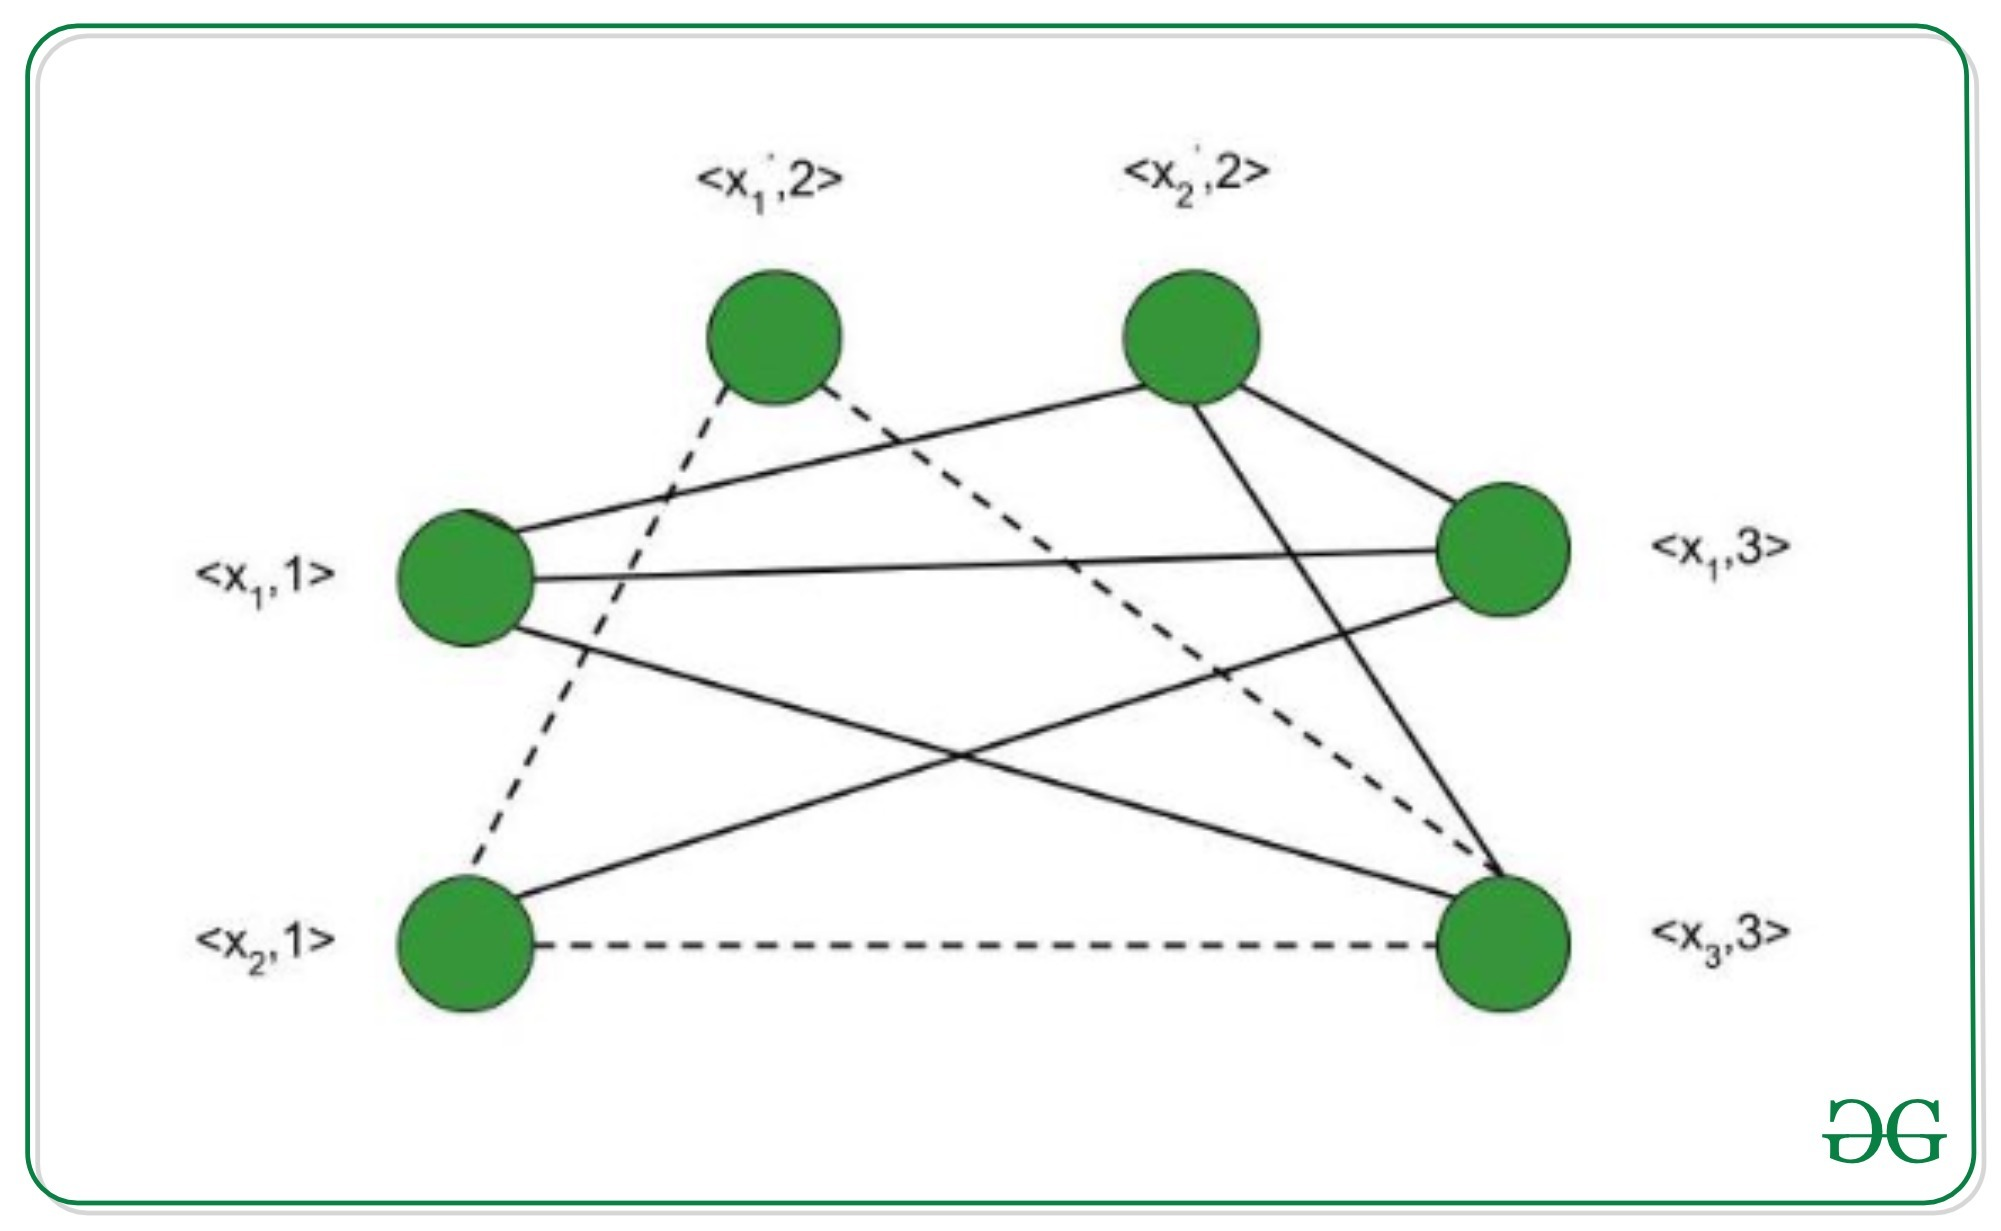
\includegraphics[width=0.5\linewidth]{images/cliqueproblem.jpeg}
            \caption{Граф, построенный по указанным правилам}
            \label{ris:cliqueproblem}
        \end{figure}
    \begin{Def}[Задача INDEPENDENT SET]
        Задача INDEPENDENT SET заключается в нахождении множеств  вершин в графе размера $k$, никакие две вершины из которых не являются смежными. Decision problem вопрос можно поставить следующим образом: существует ли множество определенного размера.
    \end{Def}
    \begin{Thm}
        Задача INDEPENDENT SET является NP-полной. 
    \end{Thm}
    \begin{proof}
        Доказательство принадлежности к классу NP оставляем в качестве упражнения читателям. Доказательство принадлежности к классу NP-hard легко проделать, изучив доказательство теоремы выше. Обратите внимание на замечание после предыдущей теоремы, поскольку оно важно.
    \end{proof}
    
    \Subsection{Определение FPT-алгоритмов. Примеры FPT-алгоритмов для VERTEX COVER и CLIQUE}
    
    \begin{Def}[FPT-алгоритм]
        Параметризированная задача P считается разрешимой с фиксированным параметром, или FPT-разрешимой (Fixed-Parameter Tractable), если она может быть решена некоторым параметризированным алгоритмом за время
        $$t(n, k) = O(n^{O(1)} * f(k))$$
        для функции $f$, зависящей только от параметра $k$.\\ 
        Порядок роста функции $f(k)$ не ограничивается. Так, возможно $f(k) = 2^{o(k)}$ или $f(k) = 2^{O(k)}$. Важно, что исключаются функции вида $f(n, k)$, например $f(n, k) = n^k$.
    \end{Def}
    \begin{Rem}
        Класс всех разрешимых с фиксированным параметром задач обозначается FPT. Соответствующие параметризированные алгоритмы, решающие такие задачи, называются FPT-алгоритмами.
    \end{Rem}
    \begin{Example}
        Примером FPT-разрешимой задачи может служить задача о вершинном покрытии графа (VERTEX COVER), когда параметром выступает размер покрытия. В самом деле, вершинное покрытие размера $k$ в графе $G$ с $n$ вершинами можно определить за время $O(n*2^k)$. Если в данной задаче в качестве параметра взять древовидную ширину $tw(G)$ графа $G$, то метод динамического программирования способен отыскать наибольшее вершинное покрытие за время $O(n * 2^{tw(G)}$). Следовательно, параметризация данной задачи относительно $tw(G)$ приводит к FPT-разрешимости.
    \end{Example}

    \Section{Вопрос 11}{}{Гагин Артур}
    
    \Subsection{Определение классов функций FP и \#P и класс языков PP}

    \begin{Def}[Функциональная задача и класс функций FP]
        Функциональная задача --- это вычислительная задача, в которой результат более сложный, чем у задачи принятия решения. Для функциональных проблем вывод не просто TRUE или FALSE. Разница между FP и P заключается в том, что задачи в P имеют одноразрядные ответы <<да>>/<<нет>>, в то время как задачи в FP могут иметь любой результат, который может быть вычислен за полиномиальное время. 
    \end{Def}
    \begin{Example}
        Сложение пяти чисел является проблемой FP, в то время как определение того, является ли их сумма нечетной, находится в P. 
    \end{Example}
    \begin{Def}[Класс функций \#P]
        \#P может быть эквивалентно определен в терминах верификатора. Проблема решения находится в NP, если существует полиномиально проверяемый сертификат для данного экземпляра проблемы, то есть NP спрашивает, существует ли доказательство принадлежности для входных данных, правильность которых можно проверить за полиномиальное время. Класс \#P спрашивает, сколько существует сертификатов для экземпляра задачи, корректность которых можно проверить за полиномиальное время. 
    \end{Def}
    \begin{Example}
        Задача определения для данного графа $G$ и числа $k$, содержит ли граф независимое множество размера $k$, находится в $NP$. Учитывая пару $(G, k)$ в языке, сертификат представляет собой набор из $k$ вершин, которые попарно несмежны (и, следовательно, являются независимым набором размера $k$). Проверка сертификата является решением NP задачи. Подсчет количества возможных сертификатов является задачей \#P.
    \end{Example}
    \begin{Def}[Класс PP]
        PP — это класс проблем принятия решений, решаемых вероятностной машиной Тьюринга за полиномиальное время с вероятностью ошибки менее 1/2 для всех случаев. 
    \end{Def}
    \begin{Def}[Вероятностная машина Тьюринга]
        Вероятностная машина Тьюринга - это тип недетерминированной машины Тьюринга, в которой каждый недетерминированный шаг представляет собой «подбрасывание монеты», то есть на каждом шаге есть два возможных следующих хода, и машина Тьюринга вероятностно выбирает, какой ход предпринять. 
    \end{Def}

    \Subsection{Доказательство эквивалентности FP = \#P и P = PP}
    
    \begin{Thm}
         FP = \#P тогда, и только тогда, когда P = PP.
    \end{Thm}
    \begin{proof}
        Доказательство в правую сторону очевидно из приведенных ниже теорем.\\
        Доказательство в левую сторону оставляем в качестве упражнения читателям.
    \end{proof}
    \begin{Thm}
        Если FP = \#P, то PP $\subseteq$ P.
    \end{Thm}
    \begin{proof}
        Данное доказательство содержит размышления <<на пальцах>>. Если классы FP и \#P совпадают, то мы можем находить не только решение задачи, но и находить их количество за полиномиальное время. Для последнего нам требуется проверка всех решений, поэтому мы можем найти правильное решение из PP, просто проверяя решения, пока не найдем верное. Мы можем сделать это за полиномиальное время из утверждения выше. Если мы можем найти правильное решение за полиномиальное время, то это задача также принадлежит классу P.
    \end{proof}
    
    \Subsection{Доказательство NP $\subseteq$ PP}
    
    \begin{Thm}
        NP $\subseteq$ PP.
    \end{Thm}
    \begin{proof}
    \end{proof}
    \begin{proof}
        Чтобы доказать это, покажем, что проблема NP-полной выполнимости принадлежит PP. Рассмотрим вероятностный алгоритм, который по формуле $F(x_1, x_2, ..., x_n)$ равномерно и случайным образом выбирает присваивание $x_1, x_2, ..., x_n$. Затем алгоритм проверяет, делает ли присвоение истинной формулу $F$. Если да, то выводит YES. В противном случае выводится YES с вероятностью $$\frac{1}{2} - \frac{1}{2^{n+1}}$$ и НЕТ с вероятностью $$\frac{1}{2} + \frac{1}{2^{n+1}}.$$
        Если формула невыполнима, алгоритм всегда будет выводить ДА с вероятностью $$\frac{1}{2} - \frac{1}{2^{n+1}} < \frac{1}{2}.$$ Если существует удовлетворяющее задание, оно выдаст YES с вероятностью не менее $$(\frac{1}{2} - \frac{1}{2^{n+1}}) * (1 - \frac{1}{2^n}) = \frac{1}{2} + \frac{1}{2^{n+1}} > \frac{1}{2}$$ (ровно 1/2, если он выбрал неудовлетворительное задание, и 1, если он выбрал удовлетворяющее задание, усреднение до некоторого числа, превышающего 1/2). Таким образом, этот алгоритм ставит выполнимость в PP. 
    \end{proof}

    \Section{Вопрос 12}{}{Гагин Артур}
    
    \Subsection{Замкнутость класса PP относительно дополнения}

    \begin{Thm}
        PP = co-PP.
    \end{Thm}
    \begin{proof}
        Пусть $L$ --- язык в PP, а $L^c$ --- его дополнение. По определению PP существует полиномиальный вероятностный алгоритм A со свойством, что
        $$x \in L \Rightarrow \Pr [A \ {\text{accepts}} \ x] > {\frac{1}{2}} \quad {\text{и}} \quad x \not \in L \Rightarrow \Pr [A \ {\text{accepts}} \ x] \leq {\frac{1}{2}}.$$
        Будем утверждать, что без ограничения общности первое неравенство всегда строгое; из этого утверждения можно вывести теорему: пусть $A^{c}$ является машиной, которая такая же, как $A$, за исключением того, что $A^{c}$ принимает входные данные, когда $A$ отклонила бы, и наоборот. Тогда:
        $$x \in L^{c} \Rightarrow \Pr [A^{c} \ {\text{accepts}} \ x] > {\frac{1}{2}} \quad {\text{и}} \quad x \not \in L^{c} \Rightarrow \Pr [A^{c} \ {\text{accepts}} \ x] < {\frac{1}{2}}.$$
        что подразумевает, что $L^{c}$ содержится в PP.\\
        Доказательство корректности утверждения, ссылающегося на <<без ограничения общности>>, можно найти здесь: \href{https://en.wikipedia.org/wiki/PP_(complexity)}{ссылка}.
    \end{proof}

    \Section{Вопрос 13}{}{Гагин Артур}
    
    \Subsection{Alternating Turing machine и класс AP}
    
    \begin{Def}[Переменная машина Тьюринга]
        Переменная машина Тьюринга — это недетерминированная машина Тьюринга, состояния которой делятся на два набора: экзистенциальные состояния и универсальные состояния. Экзистенциальное состояние является принимающим, если какой-то переход приводит к принимающему состоянию; универсальное состояние является принимающим, если каждый переход приводит к принимающему состоянию. (Таким образом, универсальное состояние без переходов принимает безоговорочно; экзистенциальное состояние без переходов безоговорочно отвергает). Машина в целом принимает слово, если начальное состояние принимает слово.\\
        Формально:\\
        Переменная машина Тьюринга представляет собой кортеж из 5 элементов.\\
        $M = (Q, \Gamma, \delta, q_{0}, g)$, где:\\
        $Q$ --- это конечное множество состояний;\\
        $\Gamma$ --- это конечный ленточный алфавит;\\
        $\delta : Q \times \Gamma \rightarrow {\mathcal {P}(Q\times\Gamma\times\{L,R\}})$ называется функцией перехода (L сдвигает голову влево, а R сдвигает голову вправо);\\
        $q_{0} \in Q$ --- это начальное состояние;\\
        $g : Q \rightarrow \{\wedge, \vee, \text{accept}, \text{reject} \}$ определяет тип каждого состояния.\\
        Если М находится в состоянии $q\in Q$ с $g(q) = \text{accept}$, то эта конфигурация считается принимающей, а если $g(q) = \text{reject}$, то говорят, что конфигурация отклоняется. Конфигурация $g(q) = \wedge$ считается принимающей, если все конфигурации, достижимые за один шаг, принимаются, и отклоняющей, если некоторая конфигурация, достижимая за один шаг, отклоняется. Конфигурация $g(q) = \vee$ считается принимающей, когда существует некоторая конфигурация, достижимая за один шаг, которая принимается, а отклоняющей, когда все конфигурации, достижимые за один шаг, отклоняются. Говорят, что $M$ принимает входную строку $w$, если начальная конфигурация $M$ принимается (отклоняет входную строку, если исходная конфигурация отклоняется).
    \end{Def}
    \begin{Def}[Класс AP]
        Класс AP является набором задач, решаемых с помощью переменной машины Тьюринга за полиномиальное время.
    \end{Def}
    
    \Subsection{Совпадение AP и PSPACE}
    
    \begin{Def}[Класс PSPACE]
        Класс PSPACE представляет собой набор всех задач принятия решений, которые могут быть решены машиной Тьюринга с использованием полиномиального объема памяти.
    \end{Def}
    \begin{Rem}
        Детерминированная машина Тьюринга может имитировать недетерминированную машину Тьюринга, не требуя гораздо большего пространства (даже если это может занять гораздо больше времени). Это значит, что рассуждать о классе PSPACE можно, используя как ДМТ, так и НМТ.
    \end{Rem}
    \begin{Thm}
        AP = PSPACE.
    \end{Thm}
    \begin{proof}
        Вложение AP $\subset$ PSPACE доказывается обычным образом: рекурсивный алгоритм будет работать на полиномиальной памяти. Обратное следует из теоремы о PSPACE-полноте языка TQBF (о ней написано ниже): машина сначала вычислит формулу, которая получается в результате сводимости, а затем будет выбирать набор её аргументов, чередуя $\exists$- и $\forall$-состояния.
        Более подробно здесь: \href{http://ru.discrete-mathematics.org/fall2017/3/complexity/compl-book.pdf}{ссылка}.
    \end{proof} 

    \Section{Вопрос 14}{}{Гагин Артур}
    
    \Subsection{AP-полнота задачи TRUE QUANTIFIED BOOLEAN FORMULAS}

    \begin{Def}[AP-полная задача]
        Задача из AP называется AP-полной, если любая задача из класса AP сводится к этой задаче за полиномиальное время.
    \end{Def}
    \begin{Def}[TQBF задача]
        TQBF задача заключается в поиске переменных, которые будут удовлетворять истинной булевой формуле с кванторами, где отсутствуют свободные переменные: $TQBF = \{\phi | \phi  \text{--- булева формула с кванторами}, Free(\phi) = \emptyset, val(\phi) = 1\}$.
    \end{Def}
    \begin{Example}
        $\forall x (y + x = 5)$. Здесь $y$ --- свободная переменная (поэтому формула не является истинной булевой формулой с кванторами).
    \end{Example}
    \begin{Example}
        $\exists y : \forall x (x \vee y)$ --- истинная булева формула с кванторами.
    \end{Example}
    \begin{Thm}
        TQBF задача является PSPACE-полной.
    \end{Thm}
    \begin{proof}
        Докажем, что TQBF является PSPACE задачей, а затем, что она является PSPACE-полной задачей.\\
        > Существует простой рекурсивный алгоритм для определения, находится ли QBF в TQBF (т. е. является ли формула истинной). Рассмотрим некоторую QBF:
        $Q_{1}x_{1}Q_{2}x_{2}\cdots Q_{n}x_{n}\phi (x_{1},x_{2},\dots ,x_{n}).$
        Если формула не содержит кванторов, мы можем просто вернуть формулу. В противном случае мы удаляем первый квантор и проверяем оба возможных значения для первой переменной:
        $$A=Q_{2}x_{2}\cdots Q_{n}x_{n}\phi (0,x_{2},\dots ,x_{n}),$$
        $$B=Q_{2}x_{2}\cdots Q_{n}x_{n}\phi (1,x_{2},\dots ,x_{n}).$$
        Если $Q_{1}=\exists$, то возвращаем $A\lor B$.\\
        Если $Q_{1}=\forall$, то возвращаем $A\land B$.\\
        Как быстро работает этот алгоритм? Для каждого квантора в исходном QBF алгоритм выполняет два рекурсивных вызова только для линейно меньшей подзадачи. Это дает алгоритму экспоненциальное время выполнения $O(2^n)$.\\
        Сколько места занимает этот алгоритм? В каждом вызове алгоритма он должен сохранять промежуточные результаты вычисления $A$ и $B$. Каждый рекурсивный вызов удаляет один квантор, поэтому общая глубина рекурсии линейна по количеству кванторов. Формулы, в которых отсутствуют кванторы, могут быть вычислены в логарифмическом пространстве по числу переменных. Начальный QBF был полностью количественно определен, так что кванторов по крайней мере столько же, сколько переменных. Таким образом, этот алгоритм использует $O(n + log n) = O(n)$ пространства. Это делает язык TQBF частью класса сложности PSPACE.\\
        > Чтобы показать, что TQBF является сложным для PSPACE, требуется показать, что любой язык в классе сложности PSPACE может быть сведен к TQBF за полиномиальное время. Т.е.,
        $$\forall L\in {\mathsf{PSPACE}},L\leq _{p}\mathrm{TQBF} .$$
        Доказательство этого пункта присутствует здесь: \href{https://en.wikipedia.org/wiki/True_quantified_Boolean_formula}{ссылка}.
    \end{proof}
    \begin{Rem}
        Из того, что TQBF задача является PSPACE-полной, следует AP = PSPACE (теорема выше). Поскольку эти классы равны, то AP-complete = PSPACE-complete (вполне очевидный факт).
    \end{Rem}

    \Section{Вопрос 16}{}{Гагин Артур}

    \Subsection{Арифметика Пресбургера}
    
    \begin{Def}[Арифметика Пресбургера]
        Арифметика Пресбургера — это теория первого порядка (формальное исчисление, допускающее высказывания относительно переменных, фиксированных функций и предикатов [утверждений]), описывающая натуральные числа со сложением, но в отличие от арифметики Пеано, исключающая высказывания относительно умножения.
    \end{Def}
    \begin{Def}[Аксиомы арифметики Пресбургера]
        Язык арифметики Пресбургера включает константы $0$, $1$, одну операцию $+$ и предикат равенства $=$. Аксиомы имеют вид:
        \begin{enumerate}
            \item $\neg (0 = x + 1)$
            \item $x + 1 = y + 1 \rightarrow x = y$
            \item $x + 0 = x$
            \item $(x + y) + 1 = x + (y + 1)$
            \item$ (P(0) \wedge (P(x) \rightarrow P(x + 1))) \rightarrow P(y)$, где $P$ ---  формула первого порядка включающая $0$, $1$, $+$, $=$ и одну свободную переменную $x$.
        \end{enumerate}
        Следует заметить, что (5) на самом деле не одна аксиома, а схема аксиом, представляющая бесконечное множество аксиом, по одной, для каждой формулы $P$. (5) является формализацией принципа математической индукции. Она не может быть эквивалентно заменена никакой конечной системой аксиом. Таким образом арифметика Пресбургера не является конечно аксиоматизируемой.
    \end{Def}
    \begin{Rem}
        В отличие от арифметики Пеано, арифметика Пресбургера является разрешимой теорией. Это означает, что для любого предложения на языке арифметики Пресбургера можно алгоритмически определить, является ли это предложение доказуемым из аксиом арифметики Пресбургера.
    \end{Rem}
    
    \Subsection{Необходимость расширения сигнатуры}
    
    \begin{Rem}
        Отметим сразу же, что с сигнатурой, указанной выше, элиминация кванторов невозможна. В самом деле, формула $\exists y (x = y + y)$; истинная для чётных $x$, не эквивалентна никакой бескванторной формуле. Поэтому нам нужно, прежде чем проводить элиминацию кванторов, расширить сигнатуру.
    \end{Rem}
    
    \Subsection{Формулировка теоремы об элиминации кванторов}
    
    \begin{Thm}
        Приведённый пример формулы выше подсказывает, какое расширение нам необходимо --- делимость по модулю (на константы): В $(\Z; =; <; +; 0; 1; \equiv_2; \equiv_3; ...)$ выполнима элиминация кванторов.
    \end{Thm}

    \Section{Вопрос 18}{}{Гагин Артур}
    
    \Subsection{Монадические теории натуральных чисел второго порядка}
    
    \begin{Def}[Логика первого порядка]
        Логика первого порядка --- формальное исчисление, допускающее высказывания относительно переменных, фиксированных функций и предикатов.
    \end{Def}
    \begin{Rem}
        Кванторы в логике первого порядка могут применяться только к переменным.
    \end{Rem}
    \begin{Def}[Логика второго порядка]
        Логика второго порядка является расширением логики первого порядка. Кванторы в ней могут применяться не только к переменным, но и к предикатам и функциям (также к множествам).
    \end{Def}
    \begin{Rem}
        Логика второго порядка несводима к логике первого порядка.
    \end{Rem}
    \begin{Def}[Монадическая логика второго порядка]
        Монадическая логика второго порядка (MSO) — это ограничение логики второго порядка, в котором разрешена только количественная оценка унарных отношений (т. е. множеств). То есть, кванторы могут появляться только(!) перед множествами. Таким образом, количественная оценка функций из-за эквивалентности отношений (функция может быть определена как особый вид бинарного отношения) как описано выше, также не допускается.
    \end{Def}

    \Subsection{Неразрешимость $\textbf{MSO}\text{Th}<\N; 0, 1, +, =, \in>$}
    
    \begin{Def}
        В математической логике и теории алгоритмов под разрешимостью подразумевают свойство формальной теории обладать алгоритмом, определяющим по данной формуле, выводима она из множества аксиом данной теории или нет.
    \end{Def}
    \begin{Thm}
        Проблема выполнимости для монадической логики второго порядка неразрешима.
    \end{Thm}
    
    \Section{Вопрос 19}{}{Гагин Артур}
    
    \Subsection{Конечные автоматы}
    
    \begin{Def}[Конечный автомат]
        Формально КА определяется в виде упорядоченной пятёрки элементов некоторых множеств:
        $$ A=(S,X,Y,\delta ,\lambda ),$$
        где:\\
        $S$ --- конечное множество состояний автомата;\\
        $X, Y$ --- конечные входной и выходной алфавиты соответственно, из которых формируются строки, считываемые и выдаваемые автоматом;\\
        $\delta :S\times X\rightarrow S$ --- функция переходов;\\
        $\lambda :S\times X\rightarrow Y$ --- функция выходов.
    \end{Def}
    \begin{Def}[Автоматный язык]
        Автоматный язык --- язык, распознаваемый некоторым конечным автоматом.
    \end{Def}
    
    \Subsection{Замкнутость регулярных языков относительно различных операций}
    
    \begin{Def}[Регулярный язык]
        Регулярный язык $REG$ над алфавитом $\Sigma = \{c_1, c_2, ...,c_k\}$ — множество, которое может быть получено из языков, каждый из которых содержит единственное слово --- $c_i$ или $\epsilon$, и пустого языка при помощи последовательных применений операций объединения, конкатенации или замыкания Клини и никаких других, то есть:
        \begin{itemize}
            \item Определим регулярные языки нулевого уровня как $R_0 = \{\emptyset, \{\epsilon\}, \{c_1\}, \{c_2\}, ...,\{c_k\}\}$.
            \item Регулярные языки ненулевого уровня определим рекуррентным соотношением: $R_{i + 1} = R_i \cup \{L_1 \cup L_2, L_1L_2, L^*_1 | L_1, L_2 \in R_i\}$.
            \item Тогда $REG = \bigcup_{i = 0}^{\infty} R_i$.
        \end{itemize}   
    \end{Def}
    \begin{Example}
        Звезда Клини для множества строк:\\ (``Go'', ``R'')$^* = $
        ($\epsilon$, ``Go'', ``R'', ``GoGo'', ``GoR'', ``RGo'', ``RR'', ``GoGoGo'', ``GoGoR'', ``GoRGo'', ...).
    \end{Example}
    \begin{Thm}[Теорема Клини]
        Классы автоматных и регулярных языков совпадают.
    \end{Thm}
    \begin{Thm}
        Пусть $L_1, L_2$ --- регулярные языки над одним алфавитом $\Sigma$. Тогда следующие языки также являются регулярными:
        \begin{enumerate}
            \item $L_1 \cup L_2$;
            \item $\overline{L_1}$.
            \item $L_1 \cap L_2$;
        \end{enumerate}
    \end{Thm}
    \begin{proof}
        Пройдемся по пунктам:
        \begin{enumerate}
            \item $L_1 \cap L_2$ является регулярным по определению регулярных языков.
            \item Рассмотрим автомат $A' = <\Sigma, Q_1, s_1,Q_1 \backslash T_1,\delta_1>$, то есть автомат, в котором терминальные и нетерминальные состояния инвертированы. Очевидно, он допускает те и только те слова, которые не допускает обычный автомат, а значит, задаёт язык $\overline{L_1}$. Таким образом, $\overline{L_1}$ --- регулярный.
            \item $L_1 \cap L_2 = \overline{\overline{L_1} \cup \overline{L_2}}$ --- регулярный.
        \end{enumerate}
    \end{proof}

    \Subsection{Совпадение классов языков, распознаваемых ДКА и НКА}

    \begin{Thm}
        Для всякого недетерминированного конечного автомата можно построить детерминированный конечный автомат, задающий точно такой же язык. 
    \end{Thm}
    \begin{proof}
        Вершины ДКА --- это подмножества множества вершин исходного НКА. Чтобы получить вершину ДКА (т.е. множество вершин исходного НКА), в которую осуществляется переход по данному символу из данной вершины ДКА (т.е. из множества M вершин НКА), надо объединить все вершины НКА, которые получаются всевозможными переходами по данному символу из всех вершин множества M, а затем добавить также вершины, достижимые с помощью переходов по пустой цепочке. Начальная вершина ДКА -- это объединение всех начальных вершин НКА плюс вершины, достижимые из начальных с помощью переходов по пустым цепочкам. Конечные вершины ДКА -- это подмножества вершин исходного НКА, содержащие хотя бы одну конечную вершину.\\
        Число вершин ДКА, вообще говоря, экспоненциально зависит от числа вершин исходного НКА.\\
        Таким образом, классы языков, задаваемых детерминированными и недетерминированными конечными автоматами, совпадают, и можно говорить просто об автоматных языках, т.е. языках, задаваемых конечными автоматами.
    \end{proof} 

    \Subsection{Разрешимость проблем Emptiness и Equality}
    
    \begin{Def}[Проблема Emptiness для конечного автомата]
         В общем случае проблему распознавания того, что язык конечного автомата пуст, называют проблемой пустоты для конечного автомата. 
    \end{Def}
    \begin{Thm}
        Проблема Emptiness для конечного автомата является разрешимой.
    \end{Thm}
    \begin{proof}
        Чтобы решить эту проблему, достаточно найти множество заключительных состояний автомата, достижимых из начального состояния. Так как конечный автомат — это ориентированный граф, то решить такую проблему можно, например, с помощью, поиска в ширину. Язык, допускаемый конечным автоматом, пуст тогда и только тогда, когда множество заключительных состояний, достижимых из начального состояния, пусто.
    \end{proof}
    \begin{Def}[Проблема Equality для конечных автоматов]
        Проблему распознавания того, является ли пара автоматов эквивалентной, называется проблема Equality.
    \end{Def}
    \begin{Rem}
        Автоматы называются эквивалентными, если ...
    \end{Rem}
    \begin{Thm}
        Проблема Equality для конечных автоматов является разрешимой.
    \end{Thm}

    \Section{Вопрос 20}{}{Гагин Артур}
    
    \Subsection{k-регулярные подмножества $\N^n$}
    
    \begin{Rem}
        Вообще говоря, автоматы принимают слова в произвольном алфавите. Однако множество слов всегда можно записать в какой-либо позиционной системе исчисления ($\N$). Каждое слово будет подаваться автомату по цифре в этой системе исчисления.  
    \end{Rem}
    \begin{Def}[Подмножество $\N$]
        Подмножество $\N$, принимаемое автоматом --- это закодированный в какой-либо системе исчисления язык, алфавитом которого являются цифры (автомат принимает по одной цифре). 
    \end{Def}
    \begin{Rem}
        Вообще говоря, особо не важно, принимать ли цифры слева направо, либо же справа налево (можно аккуратно доказать данный факт).
    \end{Rem}
    \begin{Rem}
        Легко обобщить определение, которые мы дали выше на подмножество $\N^m$: просто будем считать, например, что кортеж подается последовательно. Однако стоит отметить, что если числа разного размера, то меньшие необходимо доопределять нулями слева.
    \end{Rem}
    \begin{Def}[$k$-автоматные подмножества $\N$]
        Множество $K \subseteq \N$ называется $k$-автоматным ($k$-регулярным), если в алфавите $\{0, 1, ..., k - 1\}$ множество $k$-ичных записей элементов $K$ принимается некоторым автоматом.
    \end{Def}
        \begin{Def}[$k$-автоматные подмножества $\N^m$]
        Множество $K \subseteq \N^m (m > 1)$ называется $k$-автоматным ($k$-регулярным), если в алфавите $\{0, 1, ..., k - 1\}^m$ множество $k$-ичных записей элементов $K$ принимается некоторым автоматом.
    \end{Def}

    \Subsection{Формулировка теоремы Кобхема-Семёнова и её применение для доказательства невозможности построения конечного автомата}

    \begin{Def}[Мультипликативная независимость]
        Пара положительных целых чисел $a$ и $b$ называются мультипликативно независимой, если для целых чисел $n$ и $m$ $a^n = b^m$ подразумевает $n = m = 0$.
    \end{Def}
    \begin{Rem}
        Рассмотрим следующую задачу: дано подмножество $\N = \{0;1;2;3;...\}$. Обозначим его $E$. Можем ли мы найти элементарный алгоритм, который принимает элементы этого подмножества и отвергает те элементы, которые не принадлежат $E$ (под <<элементарным алгоритмом>> мы подразумеваем конечный автомат)? Кобхем дал пару ответов на этот вопрос. В 1969 году он доказал, что существование такого алгоритма глубого зависит от системы исчисления (numeration base). 
    \end{Rem}
    \begin{Thm}[Первая теорема Кобхема]
        Пусть $p$ и $q$ являются двумя мультипликативно независимыми целыми числами, которые больше или равны двум. Тогда подмножество $E \subset \N$ является как $p$-recognizable ($p$-распознаваемым), так и $q$-recognizable, тогда, и только тогда, когда $E$ --- это конечное объединение арифметических прогрессий.
    \end{Thm}
    \begin{Rem}
        Здесь ``$p$-recognizable'' означает что существует автомат, который принимает язык, который в точности состоит из разложения в системе исчисления $p$ элементов $E$.
    \end{Rem}
    \begin{Example}
        Например, множество $\{2^n; n \in \N\}$ является 2-recognizable. Так как не существует конечного объединения арифметических прогрессий, он не может быть 3-recognizable. Первая теорема Кобхема подразумевает что множество $\{2n;n \in \N\}$ является $p$-recognizable для любого $p \in \N$. Но это не говорит нам ничего о структуре recognizable множеств целых чисел. Рассмотрим следующую теорему, которая дает полное описание их структуры. 
    \end{Example}
    \begin{Thm}[Вторая теорема Кобхема]
        A set $E \subset \N$ is p-recognizable if and only if its characteristic sequence $x \in \{0,1\}^\N$ ($x_i = 1$ if and only if $i \in E$) is the image by a letter to letter morphism of a fixed point of a substitution of constant length $p$.
    \end{Thm}
    \begin{Rem}
        Пусть $d \geq 1$. Будем обозначать $(x_1, ..., x_d) \in \N^d$ в системе исчисления $p$ как кортеж слов над алфавитом $\{0, 1, ..., p - 1\}^d$ (с добавлением нулей в начале, если это необходимо). Например, в системе исчисления с основанием два мы запишем пару $(1,5)$ как $(0,1), (0,0), (1,1)$. Будем говорить, что $E \subset \N^d$ является $p$-recognizable если $E$, записанное в системе исчисления с основанием $p$ распознается некоторым конечным автоматом.
    \end{Rem}
    \begin{Thm}[Теорема Кобхема-Семенова]
        Пусть $p$ и $q$ --- пара мультипликативно независимых целых чисел, которые больше или равны двум. Множество $E \in \N^d$ является одновременно $p$-recognizable и $q$-recognizable тогда, и только тогда, когда $E$ является полулинейным множеством (semilinear).\\
        %, где <<полулинейное>> означает, что существует $n \in \N$ и конечные множества $V_i \subset \N^d$ ($0 \leq i \leq n$) such that
        В другой формулировке, можно считать, что теорема звучит следующим образом:\\
        пусть множество $E \subseteq \N^m$ определимо по отдельности в $<\N; 0; 1; +; V_k; =>$ и $<\N; 0; 1; +; V_l; =>$ (смотрите об этом ниже), где $k$ и $l$ мультипликативно независимы. Тогда $E$ определимо в $<\N; 0; 1; +; =>$ (в арифметике Пресбургера).
    \end{Thm}

    \Subsection{Доказательство того факта, что всякое отношение, выразимое в $<\N; 0, 1, +, V_k , =>$, является k-регулярным}
    
    \begin{Def}[Функция $V_k$]
        Определим функцию $V_k$ следующим образом:\\
        > $V_k(x) = t$, где $t$ --- максимальное значение числа $k$ в какой-либо натуральной степени, на которое делится $x$, если $x > 0$;\\
        > $V_k(x) = 1$, если $x = 0$.
    \end{Def}
    \begin{Example}
        Рассмотрим $V_2$: 
        \begin{itemize}
            \item $x = 0$: $V_2(0) = 1$;
            \item $x = 1$: $V_2(1) = 2^0$, поскольку максимальная степень $2$, на которую делится $1$ является нулем;
            \item $x = 2$: $V_2(2) = 2^1$;
            \item $x = 3$: $V_2(3) = 2^0$;
            \item $x = 4$: $V_2(4) = 2^2$;
            \item $x = 5$: $V_2(5) = 2^0$;
            \item $x = 6$: $V_2(6) = 2^1$, поскольку $6$ делится на $2^1$;
            \item $x = 7$: $V_2(7) = 2^0$;
            \item $x = 8$: $V_2(8) = 2^3$;
            \item и так далее...
        \end{itemize}
    \end{Example}
    \begin{Rem}
        $V_k$ можно трактовать как двухместный предикат, однако в виде функции это понимается проще.
    \end{Rem}
    \begin{Def}[Арифметика Бюхи]
        $<\N; 0; 1; +; V_k; =>$ --- элементарная теория структуры, называемая арифметикой Бюхи.
    \end{Def}
    \begin{Rem}
        Для разных $k$ получаются разные арифметики.
    \end{Rem}
    \begin{Thm}
        Пусть $k \geq 2$ --- натуральное число, $E \subseteq \N^m$ --- подмножество кортежей натуральных чисел. Тогда следующие утверждения эквивалентны:
        \begin{itemize}
            \item $E$ $k$-распознается некоторым конечным автоматом $A$ (является $k$-регулярным подмножеством);
            \item $E$ определимо в арифметике Бюхи с параметром $k$.
        \end{itemize}
    \end{Thm}

\end{document}